\documentclass[spanish,a4paper,12pt]{article}
\usepackage[utf8]{inputenc}
\usepackage[T1]{fontenc}
\usepackage[spanish]{babel}
\usepackage{csquotes}
\usepackage{amsmath,amssymb}
\usepackage{newtxtext,newtxmath}
\usepackage{derivative,siunitx}
\usepackage[margin=2.5cm]{geometry}
\usepackage[dvipsnames]{xcolor}
\usepackage{graphicx,float}
\usepackage[export]{adjustbox}
\usepackage[font=footnotesize,labelfont=bf]{caption}
\usepackage{subcaption,booktabs,multirow,longtable,pdflscape,chngcntr}
\usepackage[backend=biber,sorting=none]{biblatex}
\addbibresource{../../Tesis - Latex/bibliografia.bib}
\addbibresource{bibliografia_adicional.bib}
\usepackage[pdfencoding=auto,psdextra]{hyperref}
\graphicspath{{../../Tesis - Latex/}{../../}{./}}
\setlength{\parskip}{2mm}
\counterwithin{figure}{section}
\counterwithin{table}{section}
\counterwithin{equation}{section}
\makeatletter
\newcommand*{\centerfloat}{\parindent\z@\leftskip\z@\@plus1fil\@minus\textwidth
\rightskip\leftskip\parfillskip\z@skip}
\makeatother
\begin{document}
\hypersetup{pageanchor=false}
\begin{titlepage}
\centering
\vspace*{2cm}
{\LARGE Borradores integrados de los capítulos 3, 5 y 6\par}
\vspace{1cm}
{\Large Asimetrías azimutales del UMD y del SD\par}
\vspace{1cm}
{\large Versión de trabajo --- 24 de septiembre de 2026\par}
\vspace{1cm}
\begin{minipage}{0.85\textwidth}
Documento para revisión del autor y sus directores. Integra el desarrollo
analítico, la distinción entre conteo y señal, y la verificación del sesgo
de selección en la muestra SD. No modifica el manuscrito de la tesis.
Los resultados del Anillo Denso se conservan en su configuración original;
el control de selección corresponde a la producción y los intervalos
declarados en el capítulo 6.
\end{minipage}
\vfill
Las notas de cambios y procedencia acompañan a los archivos fuente.
\end{titlepage}
\pagenumbering{roman}
\hypersetup{pageanchor=true}
\tableofcontents
\clearpage
\pagenumbering{arabic}
\setcounter{section}{2}
% !TEX root = vista_previa.tex
% BORRADOR INTEGRADO, 24-09-2026. No reemplaza el archivo de la tesis.
% Fuentes, alcance y correcciones respecto de versiones anteriores: 03_NOTAS.md.

\section{Fenomenología de las asimetrías azimutales en EAS}
\label{sec:fenomenologia}

La simetría circular de la distribución de partículas en el plano perpendicular al eje de una lluvia atmosférica extensa es una aproximación útil para describir su estructura lateral. Para lluvias inclinadas, sin embargo, la diferencia de recorridos hasta el suelo y la distribución de direcciones de las partículas introducen una dependencia azimutal. La modulación observada depende además de qué magnitud registra cada detector y de qué estaciones se incluyen al calcularla. Una densidad de muones incidentes, un conteo de trayectorias que interceptan un tanque y una señal Cherenkov no son observables intercambiables.

En este capítulo se desarrollan tres contribuciones: la atenuación atmosférica, la proyección geométrica del flujo y la divergencia cinemática asociada a la distribución angular de emisión. Se explicita qué parte de la respuesta geométrica de un tanque se cancela en el límite ideal de señal proporcional a la longitud de traza. Finalmente, se introduce la selección de estaciones como un condicionamiento estadístico del observable, distinto de un mecanismo que produce o transporta muones. Esta separación permite interpretar los resultados de los capítulos siguientes sin atribuir un signo del primer armónico a una causa única.

\subsection{El plano de la lluvia y las regiones temprana y tardía}
\label{subsec:simetria_ruptura}

Las posiciones de los detectores se definen sobre el terreno y se proyectan ortogonalmente sobre el plano perpendicular al eje de la lluvia, denominado \textit{plano de la lluvia}. El radio $r$ y el azimut $\phi$ utilizados en este trabajo corresponden a ese plano; $r$ no es la distancia horizontal al núcleo. La Figura~\ref{fig:plano_lluvia} muestra ambos sistemas de referencia.

\begin{figure}[H]
\centering
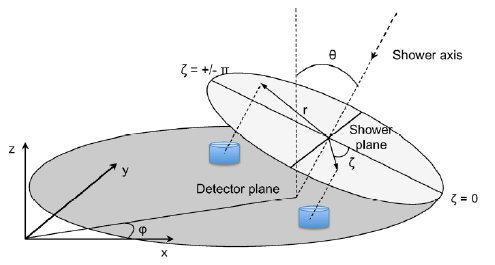
\includegraphics[width=0.7\textwidth]{capitulos/imagenes_capitulos/cap3/esquema_lluvia.png}
\caption{Proyección de las posiciones del suelo al plano perpendicular al eje de la lluvia. El azimut indicado como $\zeta$ en el esquema corresponde a $\phi$ en este trabajo.}
\label{fig:plano_lluvia}
\end{figure}

Se fija $\phi=0$ en la región \textit{temprana} y $\phi=\pm\pi$ en la región \textit{tardía}. Para una misma fuente situada sobre el eje y a igual radio $r$, el trayecto hasta el suelo es menor en el lado temprano. Los nombres identifican regiones espaciales del frente: una partícula que llega con retraso a un detector no pertenece por ello a la región tardía. En el límite de una lluvia vertical, axialmente simétrica y sin campo magnético ni anisotropías instrumentales, no existe una dirección temprano--tardía privilegiada.

Para fijar los signos se considera una fuente puntual a distancia axial $D$ del núcleo. Se aproxima el terreno por un plano horizontal y se propagan las partículas en línea recta. La geometría exacta de esta construcción es
\begin{align}
\delta&=r\tan\theta\cos\phi,&
L&=\sqrt{(D-\delta)^2+r^2},\nonumber\\
\sin\alpha&=\frac{r}{L},&
\cos\vartheta&=\frac{D\cos\theta}{L}.
\label{eq:geometria_fuente_muonica}
\end{align}
$\theta$ es el cenital de la lluvia; $L$, la distancia fuente--detector; $\alpha$, el ángulo de emisión respecto del eje descendente; y $\vartheta$, el cenital \emph{local} de la trayectoria. Se consideran puntos aguas abajo de la fuente, $D>\delta$. Entre los extremos temprano (E) y tardío (T) se cumple
\begin{equation}
L_{\mathrm T}>L_{\mathrm E},\qquad
\alpha_{\mathrm T}<\alpha_{\mathrm E},\qquad
\vartheta_{\mathrm T}>\vartheta_{\mathrm E}.
\label{eq:fen2026:orden}
\end{equation}
El desplazamiento axial involucra $r\tan\theta$, porque $r$ se define en el plano de la lluvia. Reemplazarlo por $r\sin\theta$ mezclaría esta coordenada con una distancia medida en el terreno. La fuente puntual sirve para derivar la competencia de efectos; una lluvia real requiere integrar sobre su distribución extendida de producción.

\subsection{Origen físico de la modulación azimutal}
\label{subsec:origen_fisico}

\subsubsection{Atenuación atmosférica}
\label{subsubsec:atenuacion}

Para muones con condiciones de producción equivalentes, el recorrido adicional hacia el lado tardío incrementa las pérdidas de energía, la probabilidad de decaimiento y la posibilidad de no alcanzar el detector. Estas pérdidas pasivas favorecen la región temprana. La supervivencia frente al decaimiento se escribe
\begin{equation}
P_{\mathrm{dec}}=
\exp\left[-\int_0^L\frac{\mathrm ds}{\beta(s)\gamma(s)c\tau_\mu}\right],
\label{eq:fen2026:supervivencia}
\end{equation}
donde $\tau_\mu$ es la vida media propia y la variación de $\beta\gamma$ incorpora la pérdida de energía durante la propagación~\cite{Cazon2012}. Un factor efectivo $\exp(-L/\lambda)$ representa este efecto sólo como aproximación local; no reemplaza su dependencia con la energía y la profundidad atmosférica.

La componente electromagnética ordinaria observada después del máximo de desarrollo suele ser más sensible al espesor atmosférico adicional~\cite{Pryke1998,BradfieldThesis}. No obstante, su regeneración impide identificar cualquier cambio local de densidad con absorción pura. También para los muones, una derivada de la densidad respecto de la profundidad puede contener redistribución lateral, producción adicional y cambios de la población que supera un corte energético. Por ello, no debe sumarse una ``atenuación'' deducida de esa derivada a una divergencia lateral ya calculada, salvo que ambas contribuciones hayan sido separadas.

El suelo sobre el UMD suprime fuertemente la componente electromagnética y exige a los muones un alcance suficiente para llegar al centellador~\cite{UMD_Design2016}. El filtro depende de su energía \emph{al nivel del suelo} y de su dirección local. No es un corte directo en la energía de producción, ni selecciona de manera unívoca una altura o generación de origen. Tampoco demuestra que la atenuación atmosférica domine la asimetría del UMD: la proyección geométrica puede contribuir con el mismo signo.

\subsubsection{Proyección geométrica del flujo}
\label{subsubsec:divergencia}

Las trayectorias locales no son exactamente paralelas al eje de la lluvia. En consecuencia, una superficie horizontal intercepta de forma diferente un flujo divergente en los lados temprano y tardío. Para una distribución local axialmente simétrica, el término de proyección de Bertou y Billoir se expresa como~\cite{GAP2000_017}
\begin{equation}
A_{\mathrm{geo}}(r)=
\left\langle\frac{p_r}{-p_z}\right\rangle_{\!\perp}\tan\theta,
\qquad
\mathcal A_{\mathrm{geo}}(r,\phi)=A_{\mathrm{geo}}(r)\cos\phi.
\label{eq:efecto_geo}
\end{equation}
Aquí el eje longitudinal apunta hacia arriba, de modo que $p_z<0$ para partículas descendentes, y el promedio está ponderado por el flujo de cruce del plano normal al eje. La variable $p_r$ es la componente radial \emph{con signo}, no el módulo $p_t$ del momento transversal. Para un flujo netamente saliente, $\langle p_r/(-p_z)\rangle_\perp>0$, el término es positivo y favorece la región temprana. Un momento longitudinal menor no cambia por sí mismo ese signo. Si existen trayectorias radialmente entrantes, su contribución debe determinarse con la distribución de momentos y no inferirse de que los muones tengan baja energía.

En el modelo de fuente puntual, una placa horizontal de área $A_p$ presenta a la trayectoria el área proyectada $A_p\cos\vartheta$. Como las trayectorias tempranas son más verticales, ese factor favorece el lado temprano. Esta es una modificación de la apertura frente a direcciones no paralelas, no el simple cambio de un círculo a una elipse al proyectar coordenadas. Para un haz perfectamente paralelo, una proyección consistente de posiciones y áreas no genera por sí sola ese dipolo.

\subsubsection{Divergencia cinemática y distribución angular de emisión}
\label{subsubsec:divergencia_cinematica}

Los muones producidos principalmente en decaimientos de mesones heredan una distribución de momentos longitudinales y transversales~\cite{Cazon2012}. Si $p$ es el módulo del momento inicial, $p_t=p\sin\alpha$; sólo en el límite relativista puede reemplazarse $p$ por $E_i/c$, donde $E_i$ es la energía total de producción. Para ángulos pequeños y una fuente a distancia $D$, la relación radial es $r\simeq D\alpha\simeq Dp_t/p$.

La región tardía exige un ángulo de emisión menor para alcanzar el mismo radio. Si $f(\alpha)=\mathrm dN/\mathrm d\Omega$ decrece con $\alpha$, esa región recibe partículas de una dirección más poblada de la distribución angular. Esta contribución favorece el lado tardío y es distinta de la apertura de la Ec.~\ref{eq:efecto_geo}. A la vez, el mayor recorrido tardío produce una dilución espacial mayor. Antes de incorporar apertura y supervivencia, la intensidad por unidad de área perpendicular a la trayectoria es proporcional a $f/L^2$, de modo que
\begin{equation}
\frac{[f/L^2]_{\mathrm T}}{[f/L^2]_{\mathrm E}}
=\underbrace{\left(\frac{L_{\mathrm E}}{L_{\mathrm T}}\right)^2}_{\text{favorece temprano}}
\underbrace{\frac{f(\alpha_{\mathrm T})}{f(\alpha_{\mathrm E})}}_{\text{favorece tardío si }f\text{ decrece}}.
\label{eq:fen2026:competencia}
\end{equation}
El signo neto de esta competencia no está fijado por la geometría: depende de la pendiente de la distribución angular en los ángulos que efectivamente se muestrean.

\begin{figure}[H]
\centering
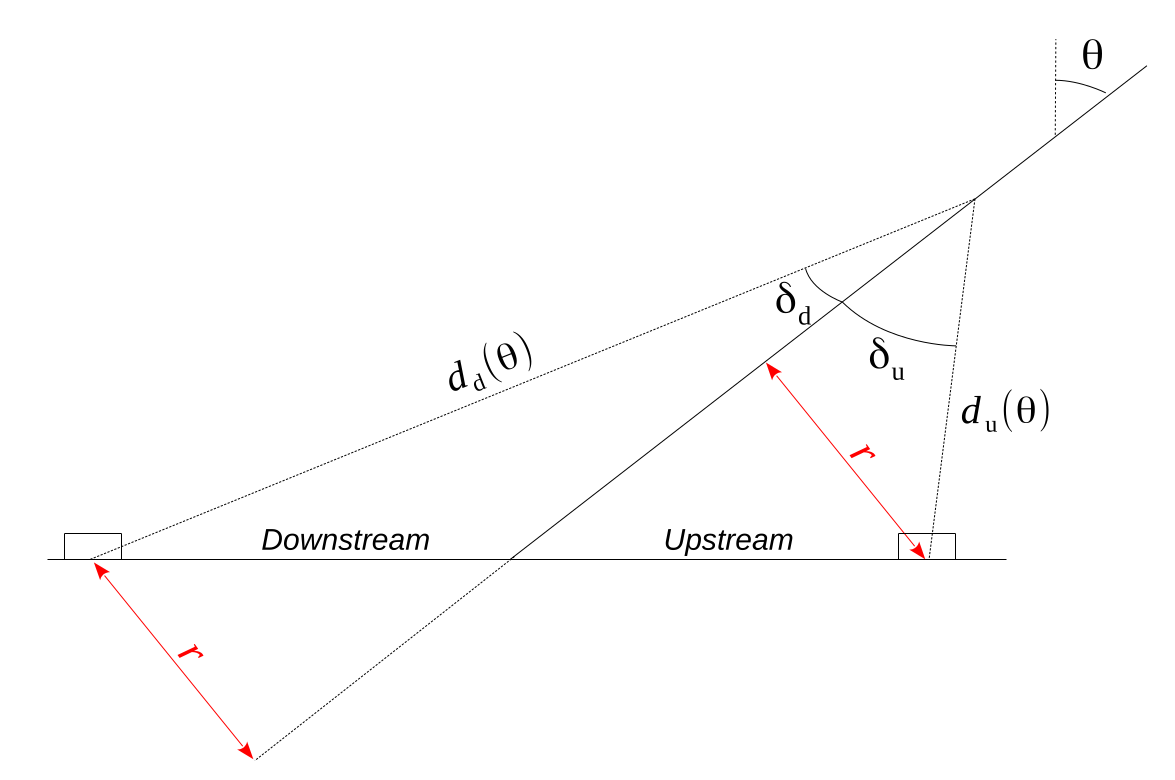
\includegraphics[width=\textwidth]{capitulos/imagenes_capitulos/cap3/efecto_geo_luce_icrc2021.png}
\caption{Geometría de la emisión hacia regiones temprana y tardía a igual radio en el plano de la lluvia. El ángulo requerido es menor hacia el lado tardío. El esquema, tomado de~\cite{Luce_ICRC2021}, ilustra la competencia angular, pero no determina por sí solo el signo del conteo o de la señal.}
\label{fig:divergencia_angular}
\end{figure}

Es posible relacionar esta pendiente con un espectro transversal, en lugar de imponer una ley de potencias angular. Como aproximación separable inspirada en el tratamiento de producción de Cazón \textit{et al.}~\cite{Cazon2012}, se considera, a momento total fijo,
\begin{equation}
g(p_t\mid p)=\frac{p_t e^{-p_t/Q}}{Q^2 Z(k)},\qquad
0\leq p_t\leq p,\qquad
k=\frac{p}{Q},\qquad
Z(k)=1-(1+k)e^{-k}.
\label{eq:fen2026:pt}
\end{equation}
$Q$ tiene unidades de momento y $Z$ normaliza el intervalo cinemáticamente permitido. Suponiendo simetría azimutal y emisión en el hemisferio delantero, $\mathrm d\Omega=2\pi\sin\alpha\,\mathrm d\alpha$ y $\mathrm dp_t=p\cos\alpha\,\mathrm d\alpha$. El cambio de variables da
\begin{equation}
f(\alpha\mid p)=
\frac{k^2}{2\pi Z(k)}\cos\alpha\,e^{-k\sin\alpha},
\qquad
\int_{\mathrm{hemisferio}}f(\alpha\mid p)\,\mathrm d\Omega=1.
\label{eq:fen2026:adf}
\end{equation}
Esta expresión es una consecuencia exacta de la aproximación de la Ec.~\ref{eq:fen2026:pt}, no el modelo completo de producción y transporte de la referencia, que incluye correlaciones entre profundidad, energía y momento transversal.

A momento fijo, el cociente de la Ec.~\ref{eq:fen2026:competencia} resulta
\begin{equation}
\frac{[f/L^2]_{\mathrm T}}{[f/L^2]_{\mathrm E}}
=\left(\frac{L_{\mathrm E}}{L_{\mathrm T}}\right)^2
\frac{\cos\alpha_{\mathrm T}}{\cos\alpha_{\mathrm E}}
\exp\left[k(\sin\alpha_{\mathrm E}-\sin\alpha_{\mathrm T})\right].
\label{eq:fen2026:cociente}
\end{equation}
Los dos factores angulares favorecen el lado tardío. A geometría y $Q$ fijos, la ganancia exponencial \emph{crece} con $p$: que los muones blandos tengan una distribución angular más ancha no implica que presenten una mayor diferencia relativa entre los dos ángulos. Una distribución ancha puede ser poco variable en el intervalo considerado; una distribución estrecha, muestreada en su cola, puede variar mucho. La ecuación no justifica atribuir automáticamente una inversión de signo a muones sub-GeV ni suprimirla mediante el umbral del UMD.

En esta contribución aislada, el cruce entre ambos extremos se obtiene
igualando el cociente a uno:
\begin{equation}
p^\ast=Q\,
\frac{2\ln(L_{\mathrm T}/L_{\mathrm E})
-\ln(\cos\alpha_{\mathrm T}/\cos\alpha_{\mathrm E})}
{\sin\alpha_{\mathrm E}-\sin\alpha_{\mathrm T}}.
\label{eq:fen2026:cruce}
\end{equation}
Si el numerador es positivo y los ángulos son distintos, existe un cruce
a momento positivo: por debajo domina el extremo temprano y por encima
el tardío. La energía total correspondiente es
$E_i^\ast=\sqrt{(p^\ast c)^2+(m_\mu c^2)^2}$.
No es un umbral universal de la lluvia ni del detector: se calculó sin
supervivencia, sin respuesta instrumental y para una sola fuente. Tampoco
equivale necesariamente al cero de un ajuste sobre todo el perfil azimutal.

Para una población con espectro inicial $G(p)$ debe calcularse el cociente de intensidades integradas,
\begin{equation}
\frac{M_{\mathrm T}}{M_{\mathrm E}}
=\frac{\int G(p)\,W_{\mathrm T}(p)\,\mathrm dp}
       {\int G(p)\,W_{\mathrm E}(p)\,\mathrm dp},
\qquad
W_j=\frac{f(\alpha_j\mid p)}{L_j^2}\,
P_j\,\mathcal R_j,\quad j=\mathrm E,\mathrm T.
\label{eq:fen2026:integrales}
\end{equation}
$P_j$ representa la supervivencia y $\mathcal R_j$ la respuesta del detector. Promediar $W_{\mathrm T}/W_{\mathrm E}$ con el espectro inicial, sin ponderar por la contribución que llega a cada región, no reproduce este cociente. Asimismo, el prefactor $k^2/Z(k)$ de la Ec.~\ref{eq:fen2026:adf} se cancela a momento fijo, pero debe conservarse dentro de cada integral. La extensión a una fuente distribuida requiere integrar también sobre la profundidad de producción y sus correlaciones.

La formulación permite verificar la consistencia del argumento cinemático, pero no constituye una predicción completa de los coeficientes medidos. En particular, extrapolar una única potencia del espectro inicial a bajas energías, omitir las pérdidas y el decaimiento, o usar un umbral al suelo como límite inferior en energía de producción modifica los pesos de la Ec.~\ref{eq:fen2026:integrales}. Una coincidencia numérica bajo esas aproximaciones no valida por sí sola una explicación del UMD.

\subsubsection{Respuesta del tanque: conteo y señal no son equivalentes}
\label{subsubsec:fen2026:tanque}

Para un cilindro vertical de radio $R$ y altura $H$, la apertura a trayectorias rectas descendentes es
\begin{equation}
\mathcal A_{\mathrm{tanque}}(\vartheta)
=\pi R^2\cos\vartheta+2RH\sin\vartheta.
\label{eq:fen2026:apertura}
\end{equation}
La tapa favorece las direcciones más verticales y el lateral las más inclinadas. Por ello, sumar las entradas laterales modifica la asimetría de un conteo calculado sólo sobre la tapa; no implica necesariamente invertir su signo~\cite{GAP2000_017}.

La señal proporcional a la longitud de traza satisface una identidad adicional. Para una dirección fija, cada punto $\mathbf b$ del área proyectada corresponde a una cuerda de longitud $\ell(\mathbf b)$ dentro del volumen. Integrar esas cuerdas reconstruye el volumen de agua:
\begin{equation}
\int_{\mathcal A_{\mathrm{proy}}}\ell(\mathbf b)\,\mathrm d^2b=V,
\qquad
\mathcal A_{\mathrm{proy}}\langle\ell\rangle=V.
\label{eq:fen2026:cuerdas}
\end{equation}
Para una fluencia $F_\perp$ uniforme sobre la escala del tanque y muones que lo atraviesan completamente, el conteo es $N_\mu=F_\perp\mathcal A_{\mathrm{proy}}$. Si cada traza produce una señal $\xi\ell$, con $\xi$ constante, entonces
\begin{equation}
S_\mu=\xi F_\perp\mathcal A_{\mathrm{proy}}\langle\ell\rangle
=\xi F_\perp V.
\label{eq:fen2026:cancelacion}
\end{equation}
La apertura y la longitud media se compensan \emph{para cada dirección}, y por tanto en cada región azimutal; no es una cancelación obtenida al promediar temprano con tardío. La identidad también puede integrarse sobre una distribución de direcciones localmente uniforme sobre el tanque.

El resultado es cero para la contribución angular de \emph{ese factor de respuesta ideal}, no para toda la asimetría muónica del SD. La señal conserva la modulación del flujo incidente $F_\perp$. El conteo de trayectorias no contiene el factor compensatorio $\langle\ell\rangle$, y los muones que se detienen, las variaciones de rendimiento luminoso, las ventanas temporales y la selección de señales requieren un tratamiento adicional. Por ello, la mayor longitud de ciertas trazas tardías no constituye por sí sola una explicación de un exceso tardío en el conteo MC. En particular, el contador de trayectorias muónicas inyectadas al tanque utilizado en esta tesis no es un conteo ponderado por la luz Cherenkov que producen.

\subsubsection{Una expresión común para los términos físicos}
\label{subsubsec:fen2026:marco}

Para una contribución rectilínea a fuente y momento fijos puede escribirse
\begin{equation}
M_d(\phi)\propto
\underbrace{P(\phi)}_{\text{supervivencia}}
\underbrace{\frac{f(\alpha(\phi))}{L(\phi)^2}}_{\text{distribución angular y dilución}}
\underbrace{\mathcal R_d(\phi)}_{\text{respuesta local}}.
\label{eq:fen2026:producto}
\end{equation}
La respuesta es $A_p\cos\vartheta$ para el conteo en una placa ideal y la Ec.~\ref{eq:fen2026:apertura} para el conteo en el tanque. Para señal ideal de muones que atraviesan el volumen, la Ec.~\ref{eq:fen2026:cancelacion} reemplaza apertura por longitud de traza integrada. La transmisión del suelo, los umbrales y las eficiencias deben incorporarse cuando corresponda. Los factores se multiplican; la suma de sus primeros armónicos es únicamente una aproximación para modulaciones pequeñas.

Esta organización recupera el resultado de Armbruster~\cite{Armbruster2018}, retomado por Luce \textit{et al.}~\cite{Luce_ICRC2021}, y precisa su observable. Si $r/D\ll1$, $\epsilon=(r/D)\tan\theta\ll1$, $f\propto\alpha^{-\gamma_{\mathrm{ADF}}}$ y $P=e^{-L/\lambda}$, resulta
\begin{equation}
A_{1,d}\simeq
\left[\underbrace{2}_{\text{dilución}}
-\underbrace{\gamma_{\mathrm{ADF}}}_{\text{pendiente angular}}
+\underbrace{D/\lambda}_{\text{atenuación}}
+\underbrace{\kappa_d}_{\text{apertura}}\right]\epsilon.
\label{eq:fen2026:bracket}
\end{equation}
Aquí $\kappa_d$ se define mediante $\mathcal R_d(\phi)=\mathcal R_{d,0}[1+\kappa_d\epsilon\cos\phi+\cdots]$, manteniendo fijos los demás parámetros. Para la placa horizontal $\kappa_d=1$; para la señal ideal de trazas completas, $\kappa_d=0$. En un conteo de intersecciones con el tanque se deriva de su propia apertura y no toma necesariamente ninguno de esos dos valores.

El $+2$ proviene exclusivamente de expandir $L^{-2}$. La expresión de señal $2-\gamma_{\mathrm{ADF}}+D/\lambda$ no incluye un $+1$ adicional de placa: en la derivación de señal, la apertura ya se compensó con la longitud media. En cambio, agregar $A_{\mathrm{geo}}$ después de multiplicar explícitamente por el área proyectada de la placa sí contaría dos veces la misma contribución.

La conexión con la distribución de la Ec.~\ref{eq:fen2026:adf} no requiere imponer una potencia global. Su pendiente local es
\begin{equation}
s(\alpha,p)\equiv-
\frac{\partial\ln f}{\partial\ln\sin\alpha}
=\tan^2\alpha+\frac{p}{Q}\sin\alpha.
\label{eq:fen2026:pendiente}
\end{equation}
En el límite de ángulos pequeños, $s$ desempeña el papel de $\gamma_{\mathrm{ADF}}$. Para una mezcla de fuentes y momentos, la pendiente efectiva debe ponderarse por las contribuciones que llegan al detector, no por el espectro de producción aislado. El término angular puede en principio superar las contribuciones positivas; por lo tanto, no existe un teorema que obligue a toda población muónica no seleccionada a tener $A_1>0$. Determinar su magnitud requiere los pesos de producción, transporte y respuesta correspondientes al observable estudiado.

\subsubsection{Campo geomagnético y dispersión durante la propagación}
\label{subsubsec:geomagnetico}

La fuerza de Lorentz, $\vec F=q\vec v\times\vec B$, desvía en sentidos opuestos a muones de cargas diferentes. La distorsión depende de la rigidez, del recorrido y de la orientación de la lluvia respecto del campo; resulta especialmente relevante en lluvias muy inclinadas~\cite{GAP2007_124,collaboration_2014}. Su eje no coincide en general con la dirección temprano--tardía. Promediar distintas direcciones de arribo puede reducir algunas contribuciones, pero no garantiza que el efecto sea nulo ni que disminuya siempre el primer armónico.

La dispersión múltiple también modifica las direcciones y posiciones de llegada, y debe distinguirse de la apertura angular adquirida en producción~\cite{Cazon2012}. Ambos procesos están fuera de la propagación rectilínea de la Ec.~\ref{eq:fen2026:producto}. No se los utiliza aquí como explicación demostrada de una inversión: aislarlos exige controles de transporte o información de partículas que permita separar su contribución. Tampoco es necesario invocar una nueva interacción atmosférica para explicar un cambio de signo que aparece al condicionar la muestra de estaciones.

\subsection{Del conteo incidente al promedio en estaciones seleccionadas}
\label{subsec:respuesta_seleccion}

Sea $\mathcal S$ la condición de retener una estación y $b$ un intervalo de radio, cenital y demás parámetros de lluvia, incluyendo el azimut. El promedio antes de imponer esa condición y el promedio seleccionado están relacionados por la identidad
\begin{equation}
\mathrm E[N_\mu\mid\mathcal S,b]
=\mathrm E[N_\mu\mid b]\,
\frac{\epsilon_{N,b}}{\epsilon_b},\qquad
\epsilon_b=P(\mathcal S\mid b),\qquad
\epsilon_{N,b}=\frac{\mathrm E[N_\mu\mathbf1_{\mathcal S}\mid b]}
                       {\mathrm E[N_\mu\mid b]}.
\label{eq:fen2026:seleccion}
\end{equation}
Los denominadores se suponen no nulos. $\epsilon_b$ es la fracción de estaciones retenidas, mientras que $\epsilon_{N,b}$ pondera esa retención por su conteo muónico. Sólo si la selección es independiente del conteo, a parámetros $b$ fijos, puede eliminarse su cociente. Una dependencia azimutal de ese cociente modifica el perfil medio y puede invertir su primer armónico. No se trata simplemente de disponer de distintas cantidades de estaciones por bin: cambia la población sobre la que se calcula la media.

En el SD, una interpretación físicamente plausible es que la mayor contribución electromagnética temprana ayude a retener tanques con pocos muones. En el lado tardío, con menor contribución electromagnética, los tanques retenidos pueden estar preferentemente enriquecidos en muones. No se crean ni se desplazan muones hacia esa región; se seleccionan estaciones con una composición de señal diferente. La atenuación electromagnética participa así indirectamente en un sesgo de selección, sin que cambie el signo temprano de las pérdidas pasivas de muones.

La Sección~\ref{subsec:control_seleccion_sd} compara los mismos conteos simulados antes y después de exigir la presencia de una estación SD reconstruida, expresada por \texttt{HasStation}. Ese control establece el cambio de signo asociado al condicionamiento en la muestra estudiada. La secuencia de ayuda electromagnética y enriquecimiento muónico anterior es una interpretación del mecanismo subyacente, no una identificación ya demostrada de un algoritmo de disparo particular ni una prueba de funcionamiento incorrecto de \textit{Offline}. El conteo puede ser de verdad Monte Carlo y, al mismo tiempo, estar sesgado por la selección de las estaciones en que se lo consulta.

El UMD no constituye un control idéntico con otro umbral. Cuenta una población transportada a través del suelo, en una superficie sensible distinta, cuyos muones no son necesariamente los que produjeron la señal del tanque asociado. La correlación de ese conteo con la selección SD puede ser diferente, aunque ambos compartan fluctuaciones de la lluvia. Una asimetría positiva del UMD no demuestra su independencia respecto de la selección, y la ausencia de información de verdad subterránea en una estación no puede reemplazarse automáticamente por un conteo físico nulo.

\subsection{Parametrización armónica y alcance de la interpretación}
\label{subsec:parametrizacion}

Siguiendo la parametrización empleada en estudios del SD~\cite{Billoir2002,BradfieldThesis}, se describe el perfil mediante
\begin{equation}
S(r,\phi)=S_0(r)\,[1+A_1(r,\theta)\cos\phi].
\label{eq:asimetria_a1}
\end{equation}
$S$ representa densidad, conteo medio o señal según se declare en cada análisis. $S_0$ es su normalización azimutal. Un coeficiente $A_1>0$ corresponde a exceso temprano y $A_1<0$ a exceso tardío; ninguno identifica exclusivamente un mecanismo. Fijar el eje en $\phi=0$ no obliga al coeficiente a ser positivo, sino que selecciona la componente temprano--tardía. Los residuos y controles complementarios permiten evaluar términos en $\sin\phi$ o armónicos superiores.

Para una modulación puramente cosinusoidal se cumple $A_1=[S(0)-S(\pi)]/[S(0)+S(\pi)]$. Fuera de ese caso, un contraste entre dos puntos, un coeficiente de Fourier y un ajuste ponderado a medias en intervalos azimutales no son necesariamente iguales. Los resultados experimentales de los capítulos siguientes se refieren al estimador declarado en la metodología, no a un contraste de dos trayectorias del modelo puntual.

En síntesis, las pérdidas pasivas y la proyección de un flujo saliente favorecen la región temprana; la preferencia angular por trayectorias más próximas al eje favorece la tardía y compite con la dilución espacial. La geometría de un tanque se compensa con la longitud media sólo para la contribución ideal a la señal de trazas completas. Finalmente, la selección modifica el promedio observado aunque los conteos individuales sean exactos. Este marco conserva los mecanismos físicos y evita usar una inversión del conteo seleccionado como prueba de una inversión de la densidad muónica incidente.

\newpage

\clearpage
\setcounter{section}{4}
% !TEX root = vista_previa.tex
% BORRADOR INTEGRADO 2026-09-24: no sustituye el archivo original.
% Conserva las figuras y etiquetas del capítulo 5. Ver 05_NOTAS.md.

\section{Caracterización de la Asimetría en el Anillo Denso}
\label{sec:cap_anillo_denso}

En este capítulo se presentan los resultados obtenidos a partir del análisis de la asimetría azimutal en la densidad de muones utilizando la configuración de \textit{Anillo Denso}. Este marco permite estudiar la respuesta del detector en condiciones de muestreo espacial controladas y reducir la mezcla vinculada a la caída radial de la densidad. La cobertura azimutal regular facilita los ajustes, aunque su precisión sigue dependiendo de la cantidad de lluvias y de las correlaciones entre estaciones. Se analizan la estabilidad de $A_1$, los efectos de reconstrucción y la sensibilidad de las amplitudes medias a la masa del primario.

\subsection{El Anillo Denso como entorno de control}
\label{subsec:entorno_control}

La configuración de Anillo Denso permite estudiar doce estaciones virtuales a un radio nominal de $r=450$~m en el plano de la lluvia. Este diseño controla la variación radial respecto del centro utilizado para construir el anillo y facilita el muestreo azimutal. No elimina por sí solo las diferencias entre el núcleo verdadero y el reconstruido ni asegura una eficiencia de selección uniforme.

Para cada observable se ajusta su media por estación o módulo en función del azimut. Se escribe genéricamente $S$ para ese observable: puede representar un conteo muónico o una señal del SD, pero no se identifican ambas magnitudes. En el anillo, los factores de área comunes no modifican la amplitud relativa. La parametrización empleada es

\begin{equation}
	S(\phi) = \langle S \rangle (1 + A_1 \cos\phi)
	\label{eq:ajuste_armonico}
\end{equation}

donde $\phi$ es el azimut en el plano de la lluvia, $\langle S\rangle$ la media azimutal y $A_1$ el coeficiente con signo. $A_1>0$ significa exceso temprano y $A_1<0$, exceso tardío. Como se discutió en el Capítulo~\ref{sec:fenomenologia}, el signo no demuestra por sí solo dominancia de atenuación o de divergencia. Tampoco se adopta un radio universal que separe regímenes dominados por cada mecanismo.

En la Figura \ref{fig:ejemplo_ajuste} se presenta un ejemplo del ajuste realizado para una muestra de protones (modelo hadrónico \texttt{Sibyll 2.3e}) en el bin de mayor inclinación ($59.3^\circ < \theta_{\text{shower}} < 65^\circ$). Los datos corresponden a la cantidad de muones reconstruida por el UMD ($N^{\text{REC}}_\mu$). Se observan las doce estaciones virtuales equiespaciadas, donde las barras de error representan la desviación estándar estadística de la media. Se aprecia una modulación clara donde la diferencia de señal entre el máximo (región temprana) y el mínimo (región tardía) es de aproximadamente un 14\% ($\pm 7\%$ respecto a la media), mostrando una modulación temprano--tardía de la componente muónica en la muestra seleccionada.

Este análisis se extendió usando también los datos de tanto la cantidad de muones inyectados en el detector y almacenados a nivel Monte Carlo ($N^{\text{MC}}_\mu$) como la señal total registrada por los detectores de superficie (SD), permitiendo contextualizar el resultado frente a estudios previos \cite{BradfieldThesis}. En estas figuras se conserva la geometría utilizada en el análisis original del anillo. En particular, el superíndice MC de un conteo identifica su origen simulado y no implica que todos los parámetros geométricos ni la selección de estaciones sean de verdad Monte Carlo.

\begin{figure}[H]
	\centering
	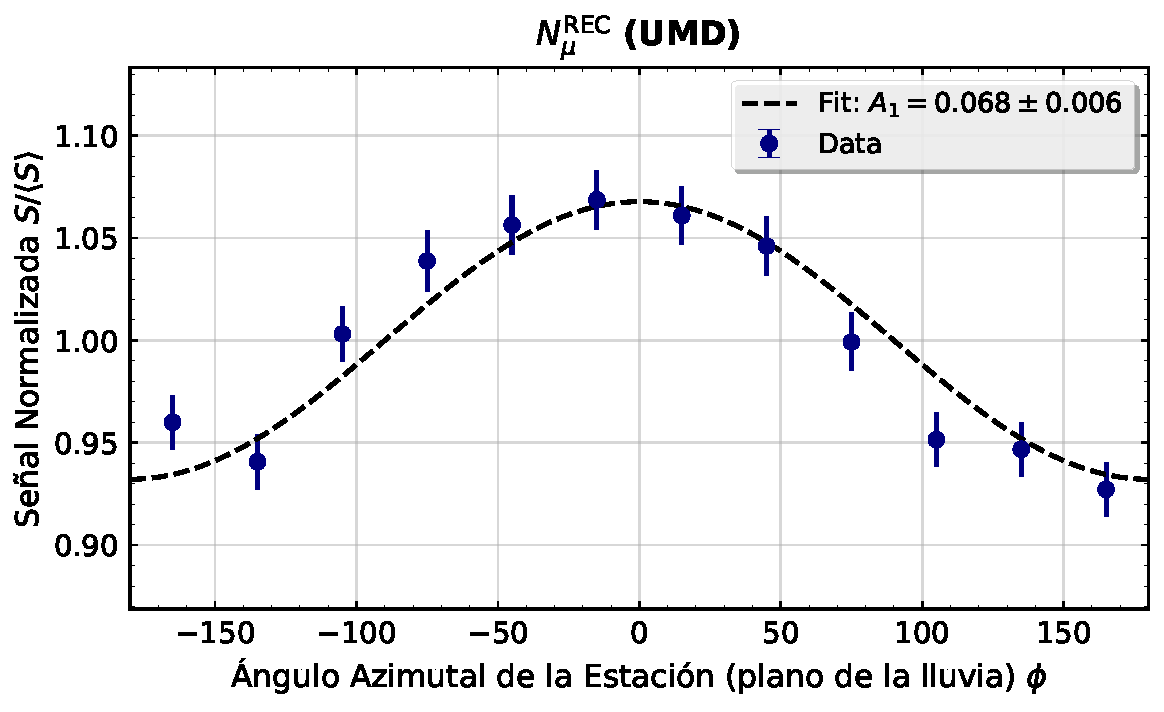
\includegraphics[width=1\textwidth]{capitulos/imagenes_capitulos/cap5/Ajuste_UMD_REC_Bin9.pdf}
	\caption{Ejemplo del ajuste armónico aplicado a la densidad de muones en el Anillo Denso para eventos de protón (\texttt{Sibyll 2.3e}). Los puntos representan las 12 estaciones virtuales y la curva sólida el ajuste del parámetro $A_1$ según la Ec. \ref{eq:ajuste_armonico}.}
	\label{fig:ejemplo_ajuste}
\end{figure}

Es importante distinguir los observables: el UMD proporciona una estimación del número de muones en el centellador, mientras que el SD registra una señal integrada calibrada en VEM (\textit{Vertical Equivalent Muon}) \cite{auger2015detector}. La unidad VEM se refiere a una respuesta de referencia del tanque; no convierte la señal total en un conteo de partículas ni en una medición calorimétrica exacta de toda la energía depositada. La evolución de $A_1$ se resume en la Figura~\ref{fig:evolucion_asym_vs_theta}.

Al comparar las curvas, el SD presenta amplitudes mayores en los bines de menor inclinación, mientras que su amplitud disminuye a partir de $\theta_{\text{shower}}\gtrsim50^\circ$. El cruce de las curvas SD y UMD no es, por sí mismo, una inversión de signo del coeficiente. 

Esta diferencia es compatible con la sensibilidad del SD a la componente electromagnética, cuyo desarrollo después del máximo es más sensible al espesor atmosférico que la supervivencia de los muones \cite{gaisser2016}. Sin embargo, la abundancia de partículas no determina por sí sola su fracción de señal: intervienen su energía y la respuesta del agua. El contraste de amplitudes es un resultado del análisis; atribuirlo cuantitativamente a atenuación, geometría o mezcla de componentes exige evaluar esos pesos.

\begin{figure}[H]
	\centering
	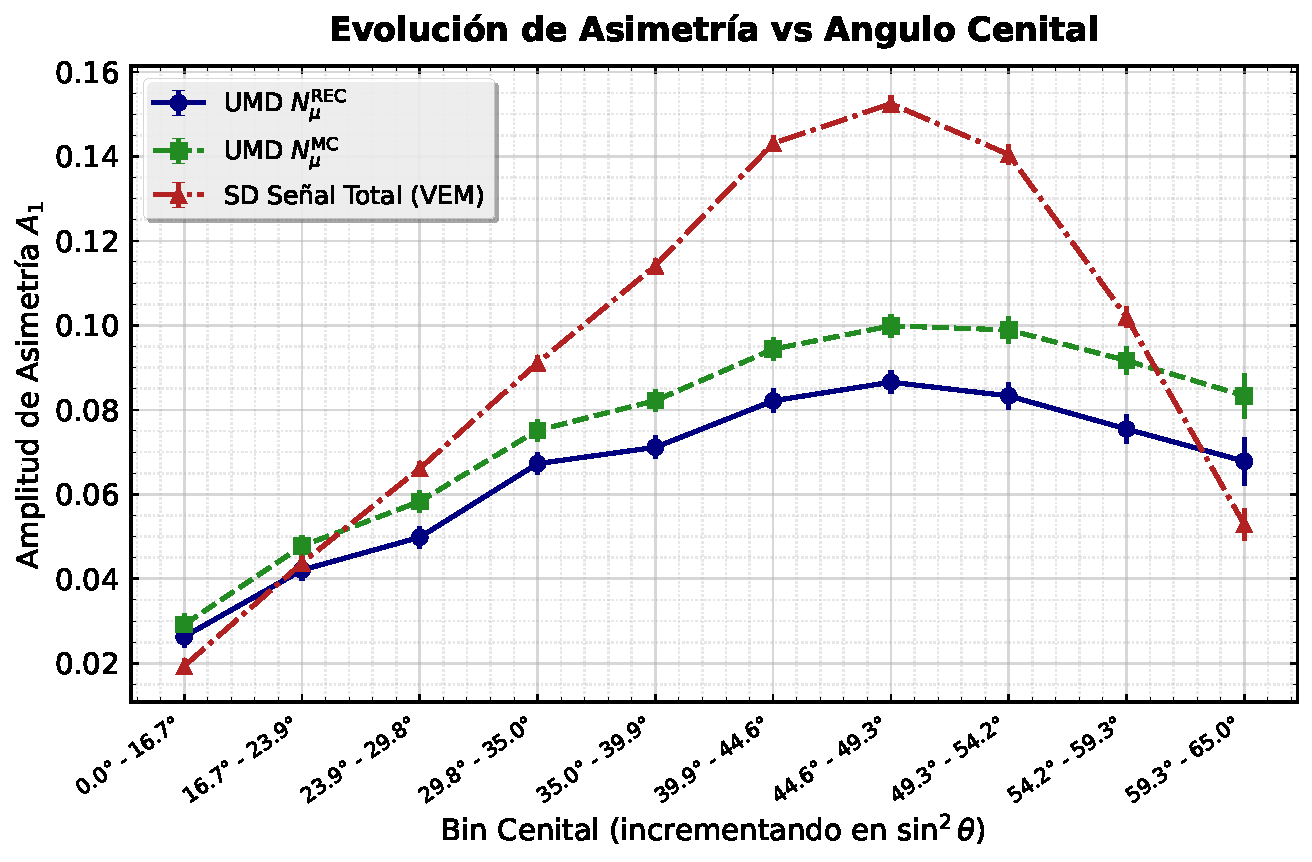
\includegraphics[width=1\textwidth]{capitulos/imagenes_capitulos/cap5/Evolucion_Asimetria_vs_Theta.pdf}
	\caption{Evolución de la amplitud $A_1$ con su error en función de $\theta$ para el UMD (REC en azul, MC en verde) y el SD (rojo). Las curvas del SD y del UMD se cruzan a altas inclinaciones. Se comparan observables distintos sobre la selección utilizada para el anillo.}
	\label{fig:evolucion_asym_vs_theta}
\end{figure}

Al aumentar la inclinación, cambia la contribución electromagnética que alcanza el suelo y, con ella, la mezcla que mide el SD. No corresponde asumir que desaparezca completamente, ni que toda reducción de $A_1$ sea causada por muones blandos dirigidos hacia la región tardía. Como muestra la Sección~\ref{subsubsec:divergencia_cinematica}, la divergencia angular y la dilución espacial compiten; el signo de su balance no se deduce de la energía baja. Además, conteo de muones, señal VEM y conteo bajo el suelo poseen aperturas y selecciones distintas. El control específico de selección del Infill, presentado en la Sección~\ref{subsec:control_seleccion_sd}, no se extrapola cuantitativamente al Anillo Denso sin una auditoría equivalente.

Finalmente, se observa una discrepancia sistemática entre los valores de asimetría $A_1$ obtenidos para los muones reconstruidos ($N^{\text{REC}}_\mu$) y los muones inyectados ($N^{\text{MC}}_\mu$) en el UMD. Esta diferencia entre observables de conteo, a menudo denominada lavado de la asimetría, se analiza en detalle en la sección \ref{subsec:mc_vs_rec}.

\subsection{Efectos Sistemáticos: Discrepancias MC vs. REC}
\label{subsec:mc_vs_rec}

Como se evidenció en la Figura~\ref{fig:evolucion_asym_vs_theta}, existe una diferencia entre las amplitudes obtenidas con muones inyectados y reconstruidos. Evaluarlas sobre las mismas estaciones y con las mismas coordenadas permite estudiar el cambio del observable asociado al conteo. No demuestra que la geometría utilizada sea exacta: un error de núcleo compartido puede afectar ambas curvas, y la respuesta de reconstrucción puede estar correlacionada con esa geometría.

En primera instancia, se evaluó la convergencia y estabilidad de los ajustes armónicos mediante la métrica de bondad de ajuste $\chi^2_\nu$. Los resultados para todos los bines cenitales se presentan en la Figura \ref{fig:chi_cuadrado_reducido}.

Para los datos del UMD, los valores de $\chi^2_\nu$ cercanos a la unidad son compatibles con una descripción armónica al nivel de precisión disponible y bajo el modelo de errores utilizado. No excluyen armónicos superiores de menor amplitud ni validan por sí solos la independencia de las medias azimutales, que comparten lluvias.

\begin{figure}[H]
	\centering
	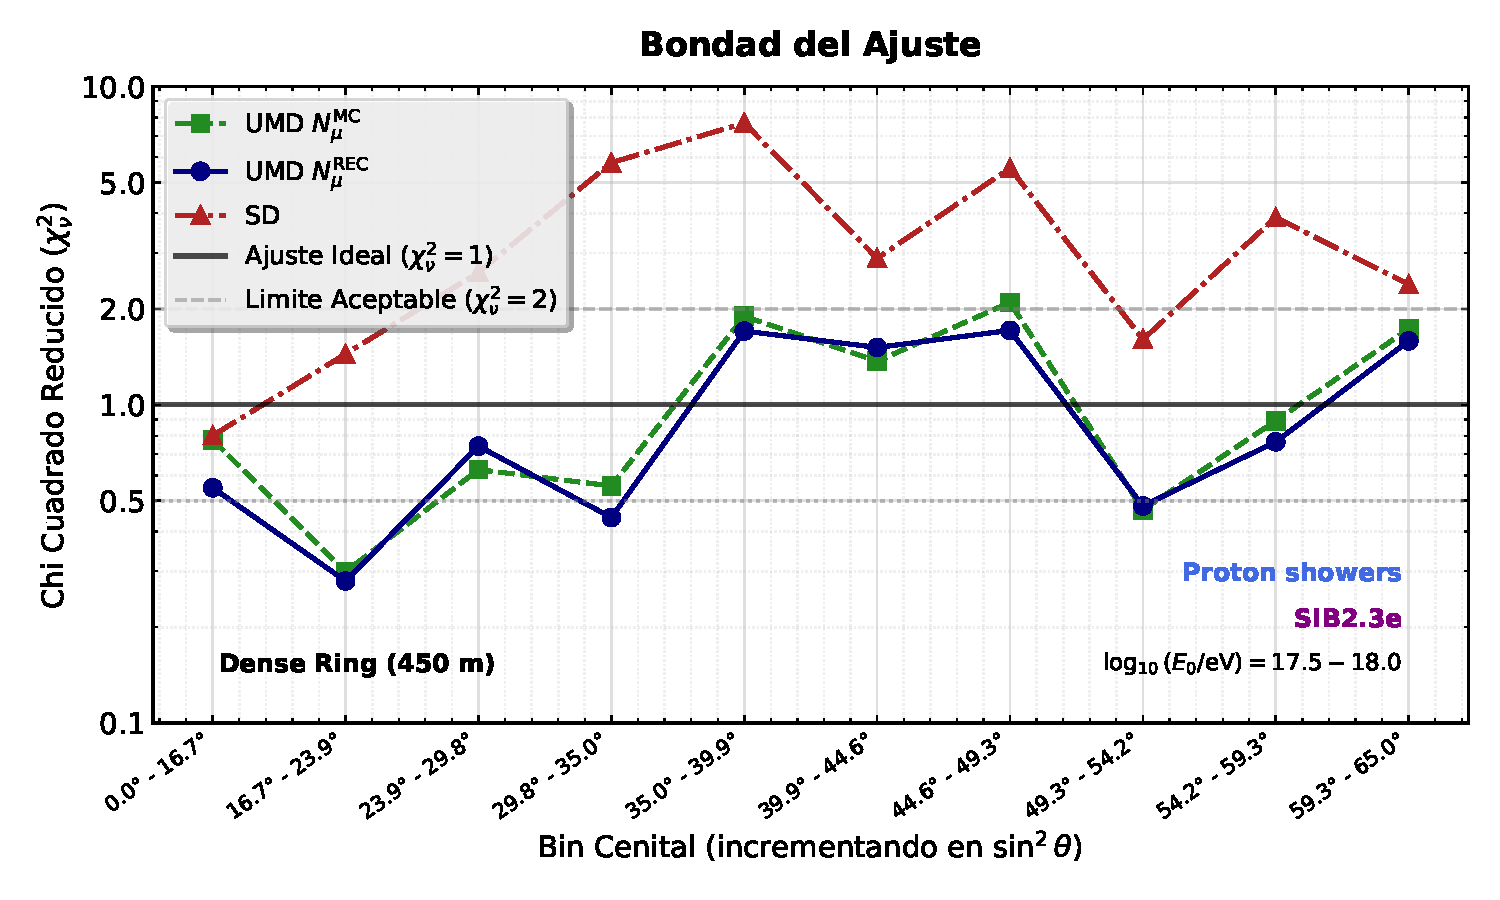
\includegraphics[width=1\textwidth]{capitulos/imagenes_capitulos/cap5/Chi2_Reduced_Fits.pdf}
	\caption{Bondad de ajuste $\chi^2_\nu$ para los bines cenitales. Los ajustes del UMD (REC y MC) se mantienen cercanos a la unidad. Los valores elevados del SD requieren revisar la descripción armónica y el modelo de errores; una alta estadística no elimina esa necesidad.}
	\label{fig:chi_cuadrado_reducido}
\end{figure}

Para el SD aparecen valores de $\chi^2/\mathrm{ndf}$ considerablemente mayores, del orden de diez en algunos intervalos. Una estadística elevada hace visibles desviaciones pequeñas, pero no vuelve irrelevante esa incompatibilidad: puede indicar estructura no representada por el primer armónico o limitaciones del modelo de incertidumbres. La inspección visual del Anexo~\ref{anexo:ajustes_anillo_denso} permite reconocer la tendencia dominante, aunque no reemplaza una prueba de residuos ni una evaluación de covarianzas.

Para investigar la discrepancia en $A_1$ dentro del UMD, se analizó el rendimiento del algoritmo de reconstrucción de muones a nivel de estación. Se definió el Residuo Relativo de Muones como:

\begin{equation}
	\varepsilon_\mu = \frac{N^{\text{REC}}_\mu - N^{\text{MC}}_\mu}{N^{\text{MC}}_\mu},\qquad N^{\text{MC}}_\mu>0.
\label{eq:dense2026_residuo}
\end{equation}

Esta métrica cuantifica el error relativo del conteo en los registros con denominador positivo. Los registros sin información de verdad Monte Carlo o con conteo nulo no admiten este residuo y no pueden incorporarse asignándoles un valor arbitrario. Además, la media de los residuos relativos no coincide en general con el residuo de las medias. La distribución de este residuo para la muestra de protones (\texttt{Sibyll 2.3e}) se muestra en la Figura \ref{fig:bias_umd_global}.

Si bien la distribución está centrada cerca del cero con una resolución aceptable, presenta una asimetría marcada respecto del cero. Mientras que el error por sub-reconstrucción está limitado físicamente (el residuo no puede ser menor a -1), el algoritmo presenta una cola de sobre-reconstrucción donde el número de muones detectados puede superar ampliamente al inyectado. La distribución documenta sobreconteos en esta muestra; no identifica por sí sola su mecanismo instrumental.

\begin{figure}[H]
	\centering
	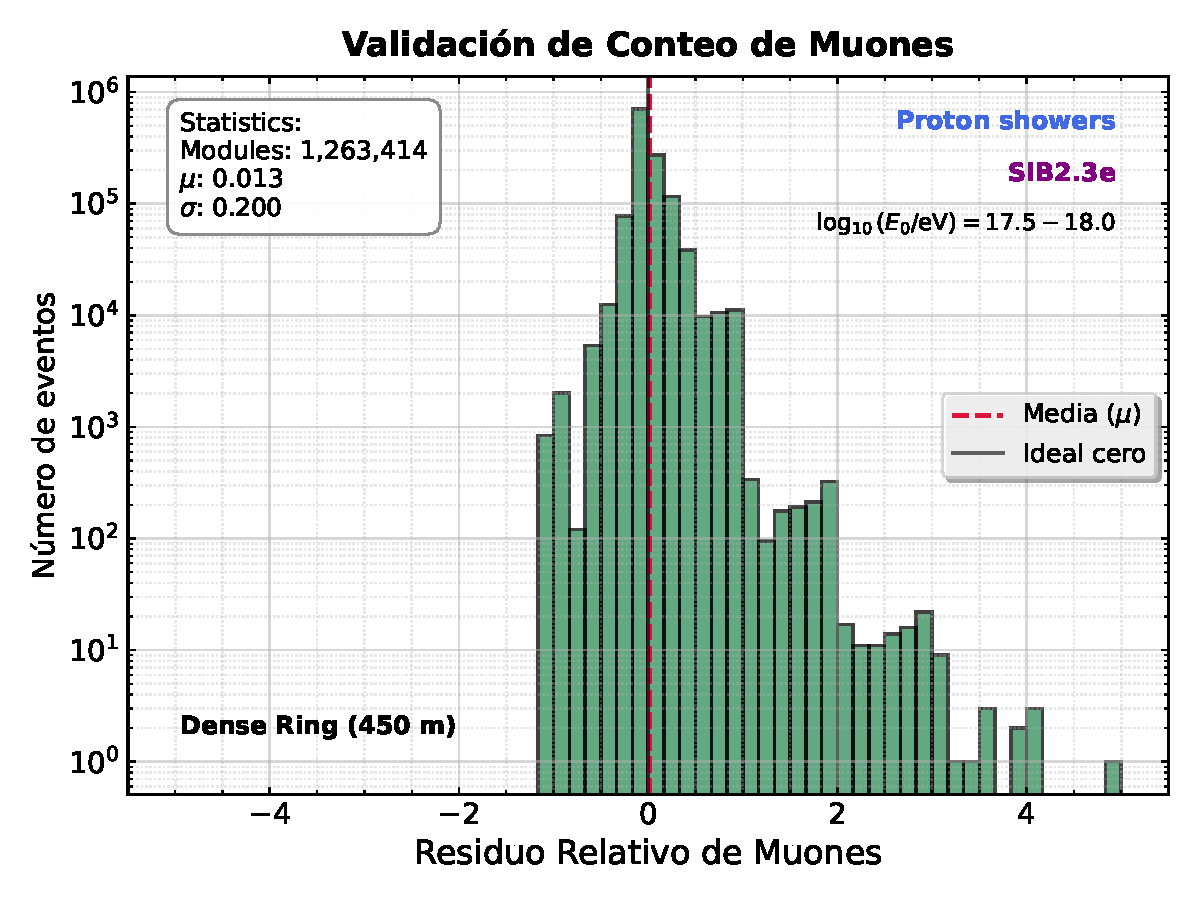
\includegraphics[width=1\textwidth]{capitulos/imagenes_capitulos/cap5/muon_counting_validation.pdf}
	\caption{Distribución del residuo relativo en la reconstrucción de muones. En los registros con conteo MC positivo se observa una cola hacia valores reconstruidos superiores a los simulados. El histograma por sí solo no identifica la causa de esa cola.}
	\label{fig:bias_umd_global}
\end{figure}

Se intentó ver si esta asimetría de la distribución respecto del cero podía explicar las diferencias de la amplitud de asimetría $A_1$ entre los datos REC y los datos MC. Para esto se construyó un modelo que implementase la distribución encontrada en la Figura \ref{fig:bias_umd_global} en los datos. Sin embargo, este procedimiento solo inyectó ruido estadístico en los ajustes, sin lograr desplazar los valores de $A_1^{\text{MC}}$ hacia los niveles de $A_1^{\text{REC}}$. Este resultado negativo sugiere que el sesgo de reconstrucción no es uniforme, sino que posee una dependencia funcional con, por ejemplo, la posición de la estación o la densidad local de partículas.

\subsubsection{Sesgo direccional en el conteo reconstruido}
\label{subsec:bias_direccional}

Se planteó la hipótesis de que el error de conteo del UMD no es uniforme, sino que presenta una dependencia con la región azimutal de la lluvia. Si el sobreconteo es proporcionalmente mayor en las zonas de baja densidad ($\phi \approx \pm 180^\circ$) que en las de alta densidad ($\phi \approx 0^\circ$), el efecto resultante sería un aumento artificial del 'piso' de la señal tardía. Esto reduciría la modulación relativa entre ambas regiones, resultando en una degradación sistemática de la amplitud $A_1$ reconstruida.

Para verificar esta premisa, se estudió la evolución del valor medio del residuo relativo para lluvias inclinadas ($40^\circ \le \theta_{\text{shower}} \le 65^\circ$) particionando la muestra en 12 bines azimutales equiespaciados en el plano de la lluvia. Los resultados se presentan en la Figura \ref{fig:bias_direccional_rec}.

\begin{figure}[H]
	\centering
	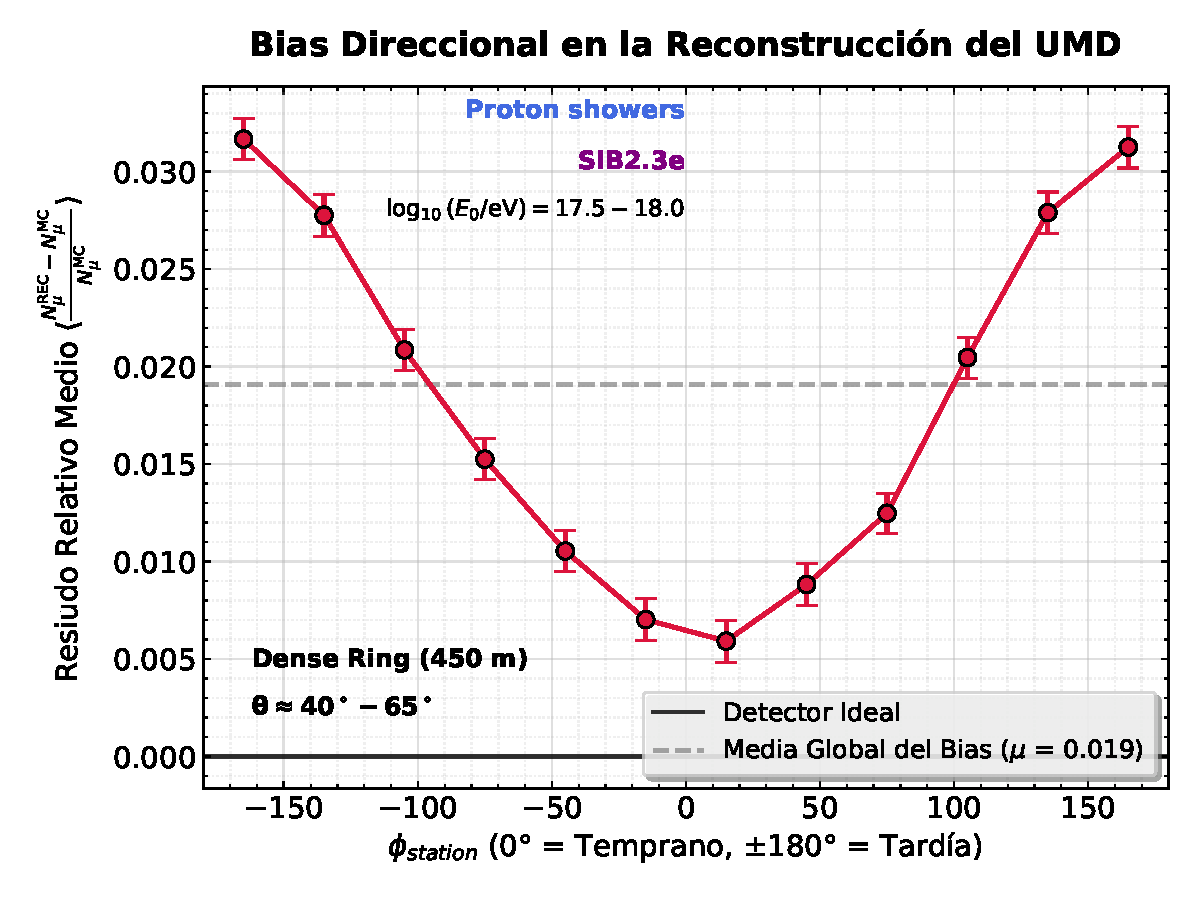
\includegraphics[width=1\textwidth]{capitulos/imagenes_capitulos/cap5/directional_bias.pdf}
	\caption{Distribución de la media del residuo relativo de reconstrucción en función del ángulo azimutal de la estación en el plano de la lluvia. El residuo relativo medio es mayor en las regiones tardías ($\pm180^\circ$) que en la región temprana ($0^\circ$), dentro de la selección analizada.}
	\label{fig:bias_direccional_rec}
\end{figure}
	
Como se observa, el residuo relativo medio es mayor en las regiones tardías de la muestra estudiada. Ese patrón es compatible con un aumento relativo del conteo tardío que reduce una modulación temprana positiva. La menor densidad puede aumentar el impacto relativo de los errores, pero la figura no aísla una causa electrónica concreta. En particular, correlaciones con ocupación, geometría y selección pueden contribuir al patrón.

\subsubsection{Transferencia empírica MC--REC: el \textit{Toy Model} de conteo}
\label{subsec:toy_model}

Para caracterizar el impacto del error de reconstrucción en la amplitud medida y verificar si el sesgo direccional es suficiente para explicar la discrepancia observada entre los datos ideales y los reconstruidos, se implementó un \textit{Toy Model} de perturbación. Este modelo utiliza un enfoque de remuestreo empírico computacional, basado en muestreo con reemplazo de los residuos observados \cite{efron1979bootstrap}. Aquí el remuestreo construye una respuesta empírica; no constituye por sí solo un cálculo de incertidumbres mediante réplicas completas de lluvias. 

El algoritmo toma las densidades muónicas ideales ($N_{\mu}^{\text{MC}}$) en cada bin azimutal y les inyecta un factor de error extraído aleatoriamente de la distribución real de residuos relativos evaluada en la Figura \ref{fig:bias_direccional_rec} segmentados por $\phi$. Esta metodología conserva dos propiedades de los residuos utilizados: respeta estrictamente el límite de sub-reconstrucción (dado que el detector no puede reconstruir cantidades negativas de muones, el residuo empírico extraído siempre está acotado en un mínimo de $-1$), y reproduce por construcción la cola asimétrica de sobreconteo característica del algoritmo del UMD. 

De esta manera, se evalúa la degradación resultante en $A_1$ considerando exclusivamente el efecto del ruido de conteo direccional, sin introducir una perturbación adicional de la posición del núcleo, permitiendo su comparación directa con la asimetría reconstruida ($A_1^{\mathrm{REC}}$). Los resultados de este modelo se observan en la Figura \ref{fig:toy_model}.

\begin{figure}[H]
	\centering
	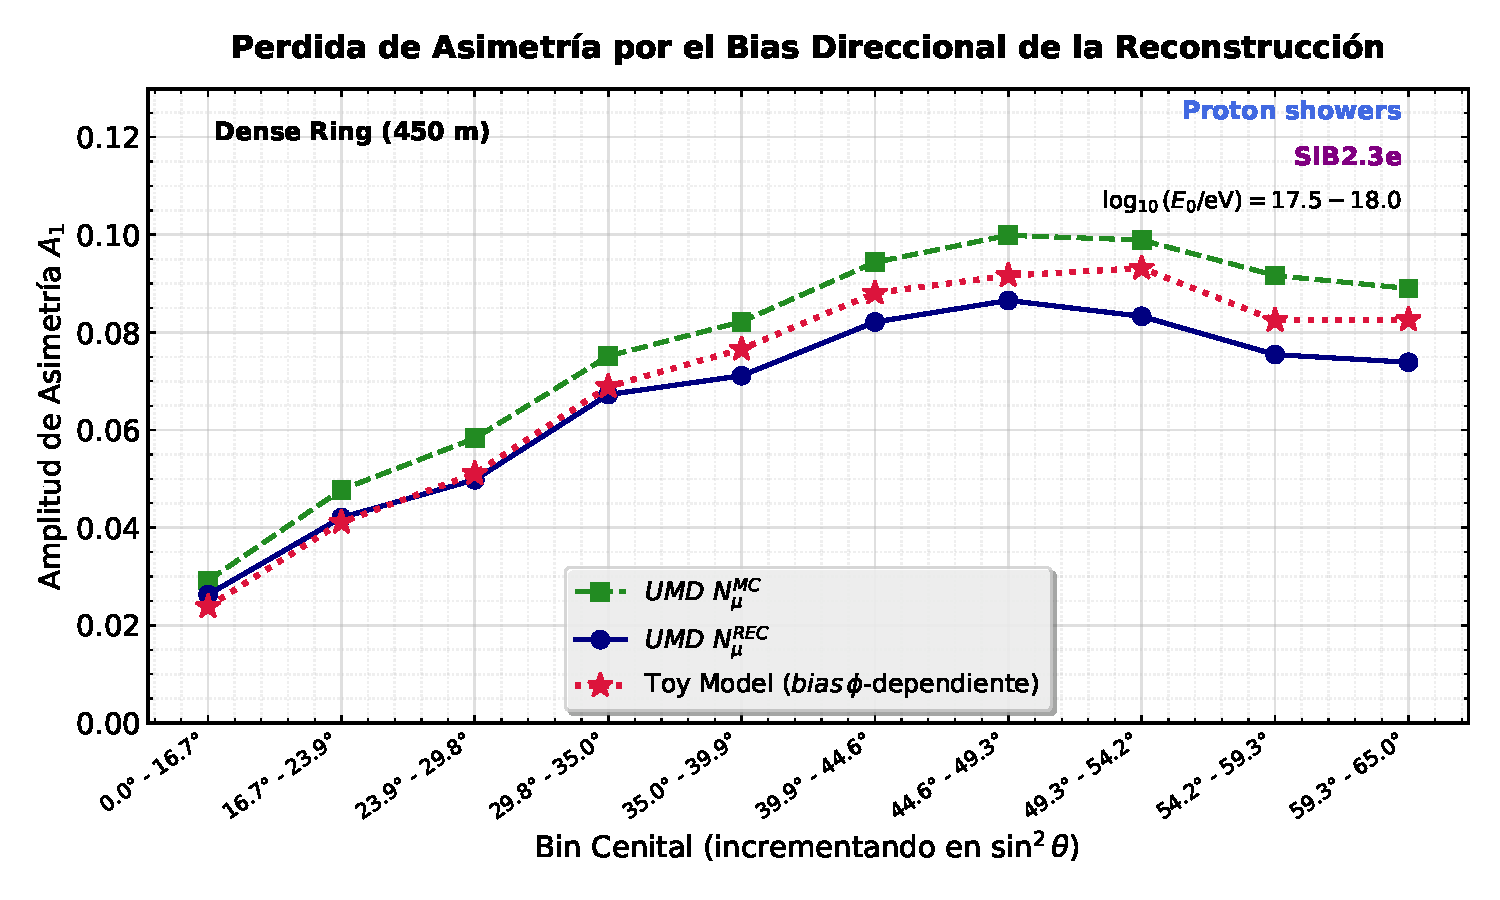
\includegraphics[width=1\textwidth]{capitulos/imagenes_capitulos/cap5/toy_model.pdf}
	\caption{Comparación de la amplitud de asimetría $A_1$ para muones inyectados (verde), reconstruidos (azul) y el resultado del \textit{Toy Model} direccional (rojo). Se aprecian dos regímenes diferenciados de degradación de señal según la inclinación de la cascada.}
	\label{fig:toy_model}
\end{figure}

La comparación muestra que el \textit{Toy Model} logra reproducir el comportamiento de los datos reconstruidos, con dos regímenes de acuerdo empírico:

\begin{itemize}
\item Para $\theta\lesssim35^\circ$, el remuestreo direccional reproduce aproximadamente la curva reconstruida. Esto demuestra la capacidad descriptiva de los residuos utilizados, no una identificación independiente de su causa.
\item Para inclinaciones mayores persiste una diferencia. El resultado indica que la transferencia empírica unidimensional no captura toda la respuesta; no identifica de forma única al núcleo, al conteo o al tratamiento de trayectorias en bordes como responsables.
\end{itemize}

La operación realizada puede resumirse como
\begin{equation}
N_\mu^{\mathrm{toy}}=N_\mu^{\mathrm{MC}}(1+\varepsilon_\mu^\ast),
\qquad
\varepsilon_\mu^\ast\sim \widehat p(\varepsilon_\mu\mid b_\phi),
\label{eq:dense2026_transferencia}
\end{equation}
donde $b_\phi$ identifica el bin azimutal y el asterisco indica un residuo remuestreado. El modelo conserva la dependencia azimutal marginal del residuo, pero no necesariamente su correlación con $N_\mu^{\mathrm{MC}}$, energía, cenital u ocupación. Por ejemplo, aun a azimut fijo,
\begin{equation}
\langle N_\mu^{\mathrm{REC}}\rangle
=\langle N_\mu^{\mathrm{MC}}\rangle
+\langle N_\mu^{\mathrm{MC}}\varepsilon_\mu\rangle,
\label{eq:dense2026_media_residuo}
\end{equation}
y el último término no es, en general, el producto de las medias. Esta distinción explica por qué transferir correctamente el histograma marginal de errores no obliga a reproducir toda la modulación.

El \textit{Toy Model} constituye así un control empírico útil de la transferencia MC--REC, distinto de un modelo de producción o propagación de muones. El acuerdo a bajas inclinaciones y la corrección parcial a inclinaciones mayores son resultados del procedimiento, no una identificación independiente de su causa. En particular, no se inyecta un desplazamiento del núcleo: el remanente no demuestra que ese desplazamiento sea el efecto faltante. Extender el modelo a geometría y ocupación requiere conservar las correlaciones pertinentes, preferiblemente con muestras separadas para construir y validar la transferencia.

\subsubsection{Sesgo geométrico y posible absorción de la asimetría por la LDF}
\label{subsec:dense2026_nucleo}

La discrepancia residual motiva examinar la geometría reconstruida. Aunque el anillo controla el radio respecto del centro empleado para construirlo, la comparación con la cascada verdadera depende de la diferencia MC--REC del núcleo. Una perturbación espacial puede mezclar simultáneamente radios y azimuts.

Para investigar la precisión geométrica de esta reconstrucción, se analizó el error en la determinación de la coordenada radial utilizando datos de las estaciones reales del \textit{Infill}. En la Figura \ref{fig:bias_core_azimut} se presenta el error radial ($\Delta r = r_{MC} - r_{REC}$) en función del azimutal verdadero de la estación ($\phi_{MC}$) en el plano de la lluvia. Se grafican solo las estaciones que se encuentra entre $r_{REC} \in [0,1400]m$ del eje de la lluvia.

La Figura~\ref{fig:bias_core_azimut} muestra una modulación de $\Delta r=r_{\mathrm{MC}}-r_{\mathrm{REC}}$. En la región temprana predomina $\Delta r<0$ y en la tardía $\Delta r>0$. A dirección fija, este patrón es compatible con un desplazamiento del núcleo reconstruido hacia el lado tardío. Si también cambian los ángulos de arribo y la selección radial, deben separarse esas contribuciones antes de interpretar la modulación como una medición exclusiva del desplazamiento del núcleo.

\begin{figure}[H]
	\centering
	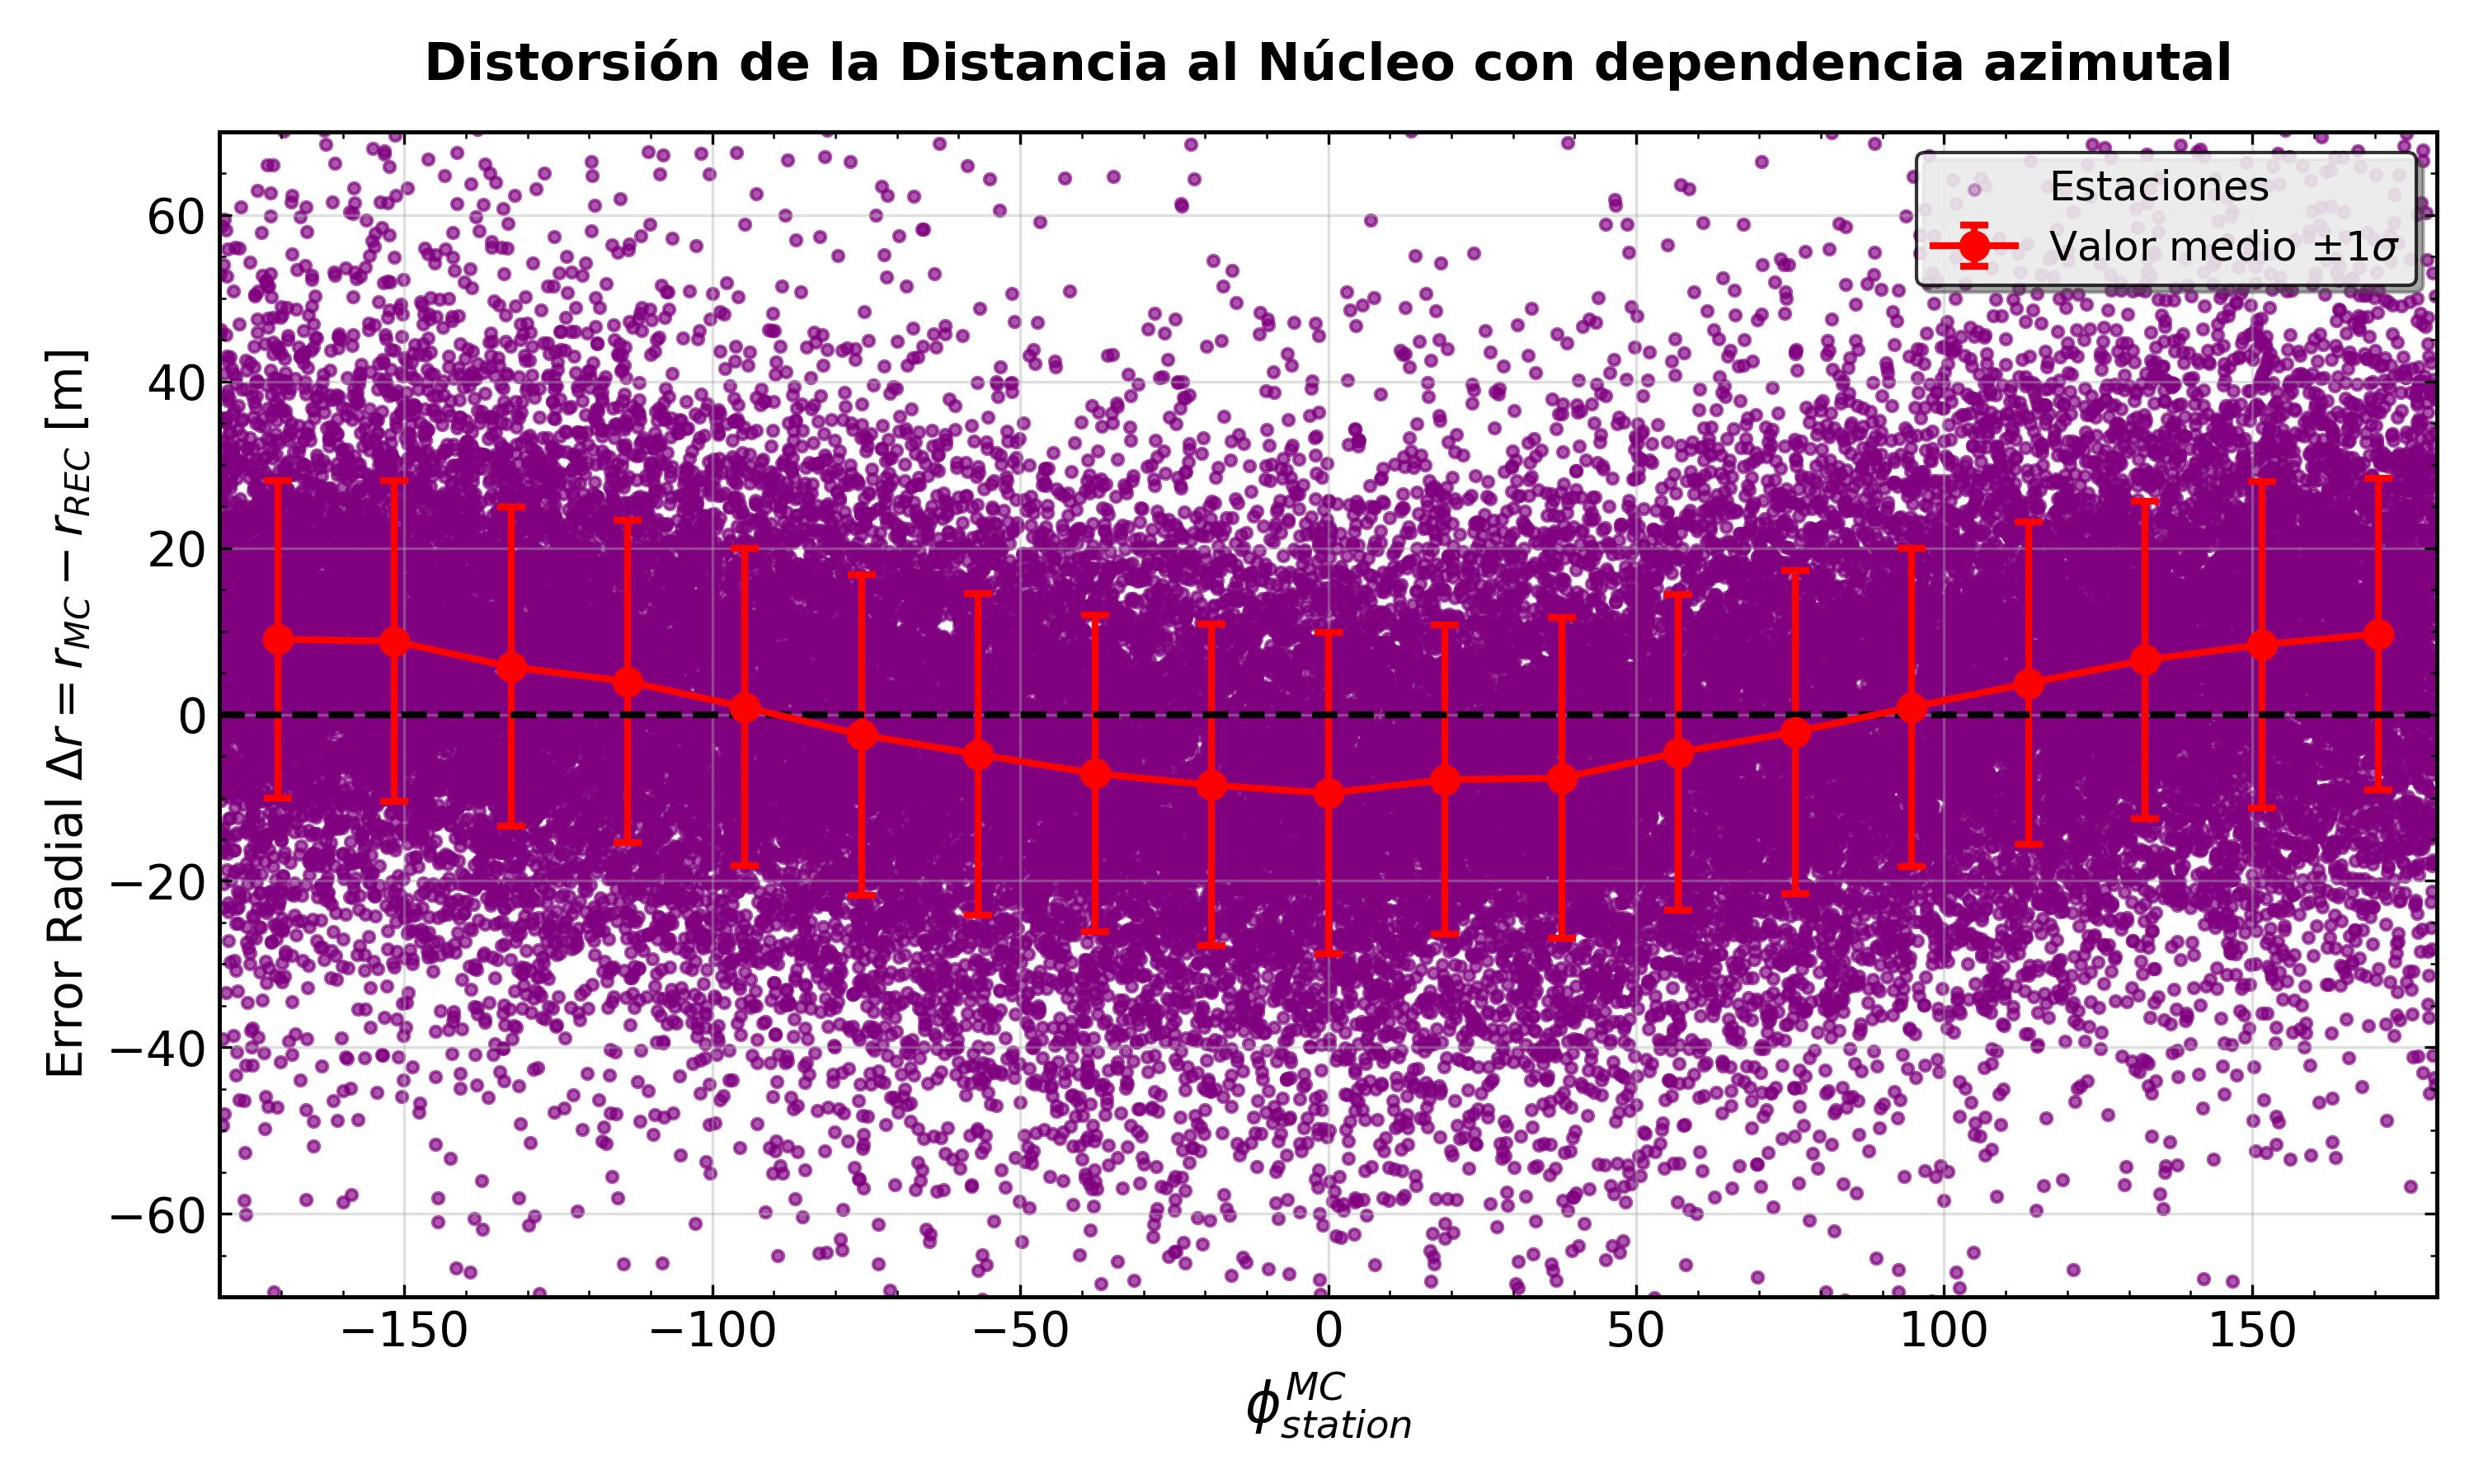
\includegraphics[width=1\textwidth]{capitulos/imagenes_capitulos/cap5/error_radial_azimut.jpg}
	\caption{Distorsión de la coordenada radial de las estaciones del \textit{Infill} en función del ángulo azimutal. La modulación es compatible con un componente sistemático del error geométrico a lo largo del eje temprano--tardío; no identifica por sí sola su origen.}
	\label{fig:bias_core_azimut}
\end{figure}

La relación geométrica puede explicitarse manteniendo fija la dirección de la lluvia. Sea $\boldsymbol\delta=\boldsymbol x_{\mathrm{core,REC}}-\boldsymbol x_{\mathrm{core,MC}}$ el desplazamiento en el plano transversal y $\widehat{\boldsymbol r}(\phi)$ la dirección de la estación medida desde el núcleo verdadero. Para $|\boldsymbol\delta|\ll r$,
\begin{equation}
r_{\mathrm{REC}}\simeq r_{\mathrm{MC}}
-\boldsymbol\delta\cdot\widehat{\boldsymbol r}(\phi),
\qquad
\Delta r\simeq\boldsymbol\delta\cdot\widehat{\boldsymbol r}(\phi).
\label{eq:dense2026_corrimiento}
\end{equation}
Un desplazamiento hacia el lado tardío da $\Delta r<0$ en el lado temprano y $\Delta r>0$ en el tardío, de acuerdo con el patrón mostrado. La misma expansión introduce un término angular al evaluar una LDF radial:
\begin{equation}
S_0(r_{\mathrm{REC}})\simeq S_0(r_{\mathrm{MC}})
-\frac{dS_0}{dr}\,
\boldsymbol\delta\cdot\widehat{\boldsymbol r}(\phi).
\label{eq:dense2026_degeneracion_ldf}
\end{equation}
Esta identidad demuestra una degeneración local entre primer armónico y posición del núcleo; no determina por sí sola qué desplazamiento elegirá el ajuste real.

Una LDF radial sin modulación azimutal puede absorber parte de una asimetría mediante cambios en el núcleo, la pendiente o la normalización. Esta degeneración constituye una explicación posible del patrón, pero no demuestra que el ajustador esté respondiendo a un exceso intrínseco de muones blandos en la región tardía. Tampoco implica que el conteo local del UMD sea modificado explícitamente para forzar una LDF.

El desplazamiento del núcleo puede cambiar la asignación de radios y azimuts y, de ese modo, el armónico extraído. Para determinar cuánto de la diferencia MC--REC se debe a este efecto sería necesario repetir el análisis sobre las mismas estaciones alternando únicamente la geometría, o comparar reconstrucciones con parametrizaciones simétrica y asimétrica. La modulación radial y el remuestreo direccional aportan controles complementarios, pero no cierran por sí solos la cadena causal. Ambos deben distinguirse del requisito de presencia de una estación SD reconstruida: éste modifica qué estaciones entran en la muestra y puede afectar incluso un análisis realizado enteramente con geometría MC.

\subsection{Estudios de Robustez}
\label{subsec:robustez}

Se estudió la estabilidad del observable frente a cambios de dirección de arribo y modelo hadrónico. Estos controles buscan variaciones adicionales a las dependencias en radio e inclinación, sin asumir de antemano que deban ser exactamente nulas.

\subsubsection{Invariancia azimutal de incidencia ($\phi_{shower}$)}
\label{subsubsec:invariancia_phi}

Para asegurar que la asimetría medida sea una propiedad intrínseca de la cascada y no un artefacto de la orientación del arreglo, se evaluó la estabilidad de $A_1$ en función del ángulo azimutal de entrada de la lluvia ($\phi_{\text{shower}}$). Para esto se separaron los datos del anillo denso en 6 bines equiespaciados en función del angulo de incidencia de la lluvia y se repitio el análisis explicando en la sección \ref{subsec:entorno_control} para cada uno de ellos.

 \begin{figure}[H]
	\centering
	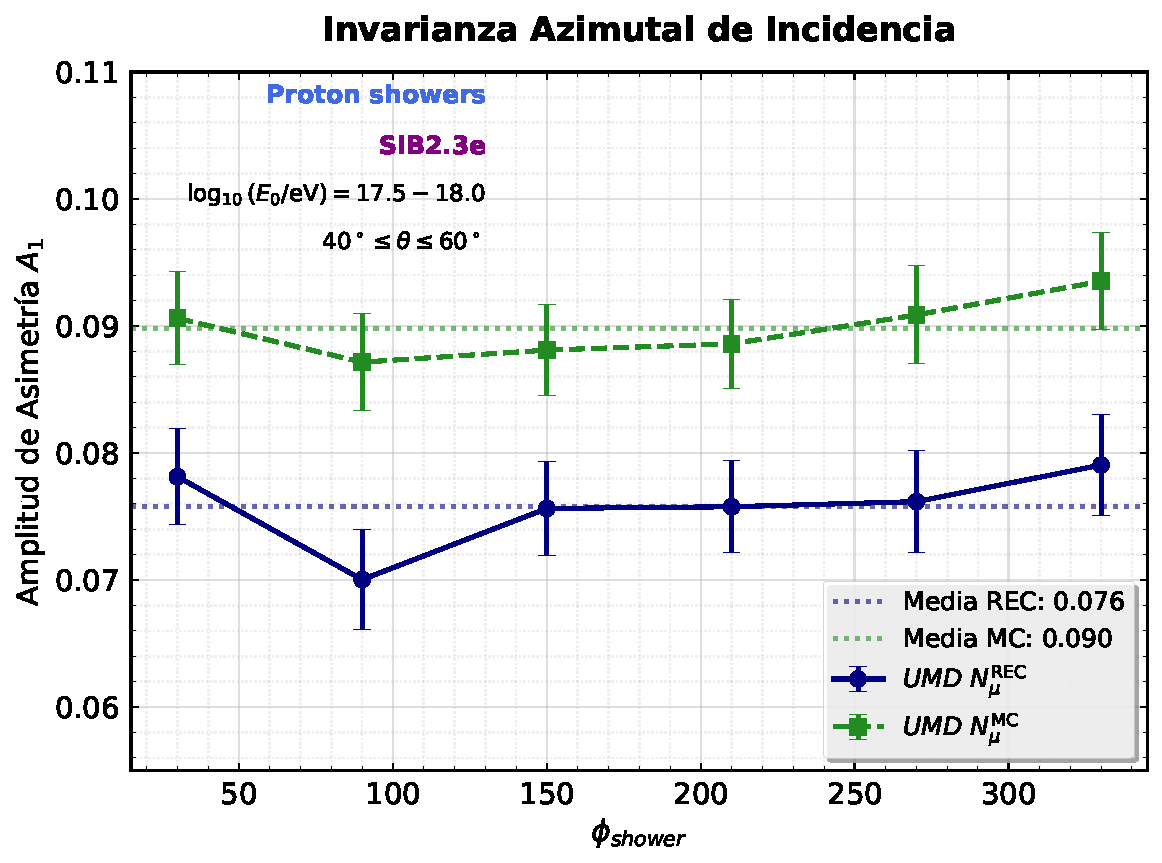
\includegraphics[width=1\textwidth]{capitulos/imagenes_capitulos/cap5/DenseRing_Systematics_Isotropy.pdf}
	\caption{Amplitud $A_1$ en función del ángulo azimutal de la lluvia. No se aprecia una dependencia marcada con la dirección de arribo a la precisión de la comparación.}
	\label{fig:robustez_phi}
 \end{figure}

En la Figura~\ref{fig:robustez_phi}, para protones de \texttt{SIBYLL 2.3e} y $40^\circ<\theta<60^\circ$, no se aprecia una dependencia marcada con el azimut de arribo a la precisión de la comparación. Este resultado apoya la estabilidad del análisis en esa muestra; no excluye toda contribución geomagnética ni toda dependencia instrumental con la orientación. Persiste la diferencia entre conteos inyectados y reconstruidos.

\subsubsection{Comparación entre modelos hadrónicos}
\label{subsubsec:independencia_modelo}

Análogamente, se evaluó la robustez de la asimetría $A_1$ frente al uso de diferentes modelos de interacciones hadrónicas en las simulaciones. Para ello, se comparó la evolución del parámetro $A_1$ para un mismo primario (Helio) y rango de energía utilizando diferentes librerías fenomenológicas. Dada la disponibilidad de datos detallada en el Capítulo 4, se contrastaron las cascadas simuladas con los modelos \texttt{SIBYLL 2.3e} y \texttt{QGSJet-III.01}.

No existe una garantía teórica de independencia del modelo hadrónico: cambiar la producción modifica tanto las normalizaciones como las distribuciones de energía, altura y momento transversal que intervienen en $A_1$. Por ello, la comparación entre modelos es un control empírico, y no una consecuencia obligatoria de la cinemática.

Para llevar a cabo esta validación, se replicó el análisis angular realizando ajustes independientes por bin cenital, tal como se detalló en la sección \ref{subsec:entorno_control}. A su vez, se calculó la diferencia relativa porcentual entre los valores de amplitud obtenidos por ambos modelos, propagando las incertezas estadísticas correspondientes. La comparación de estas distribuciones se presenta en la Figura \ref{fig:modelos_hadronicos}.

\begin{figure}[H]
	\centering
	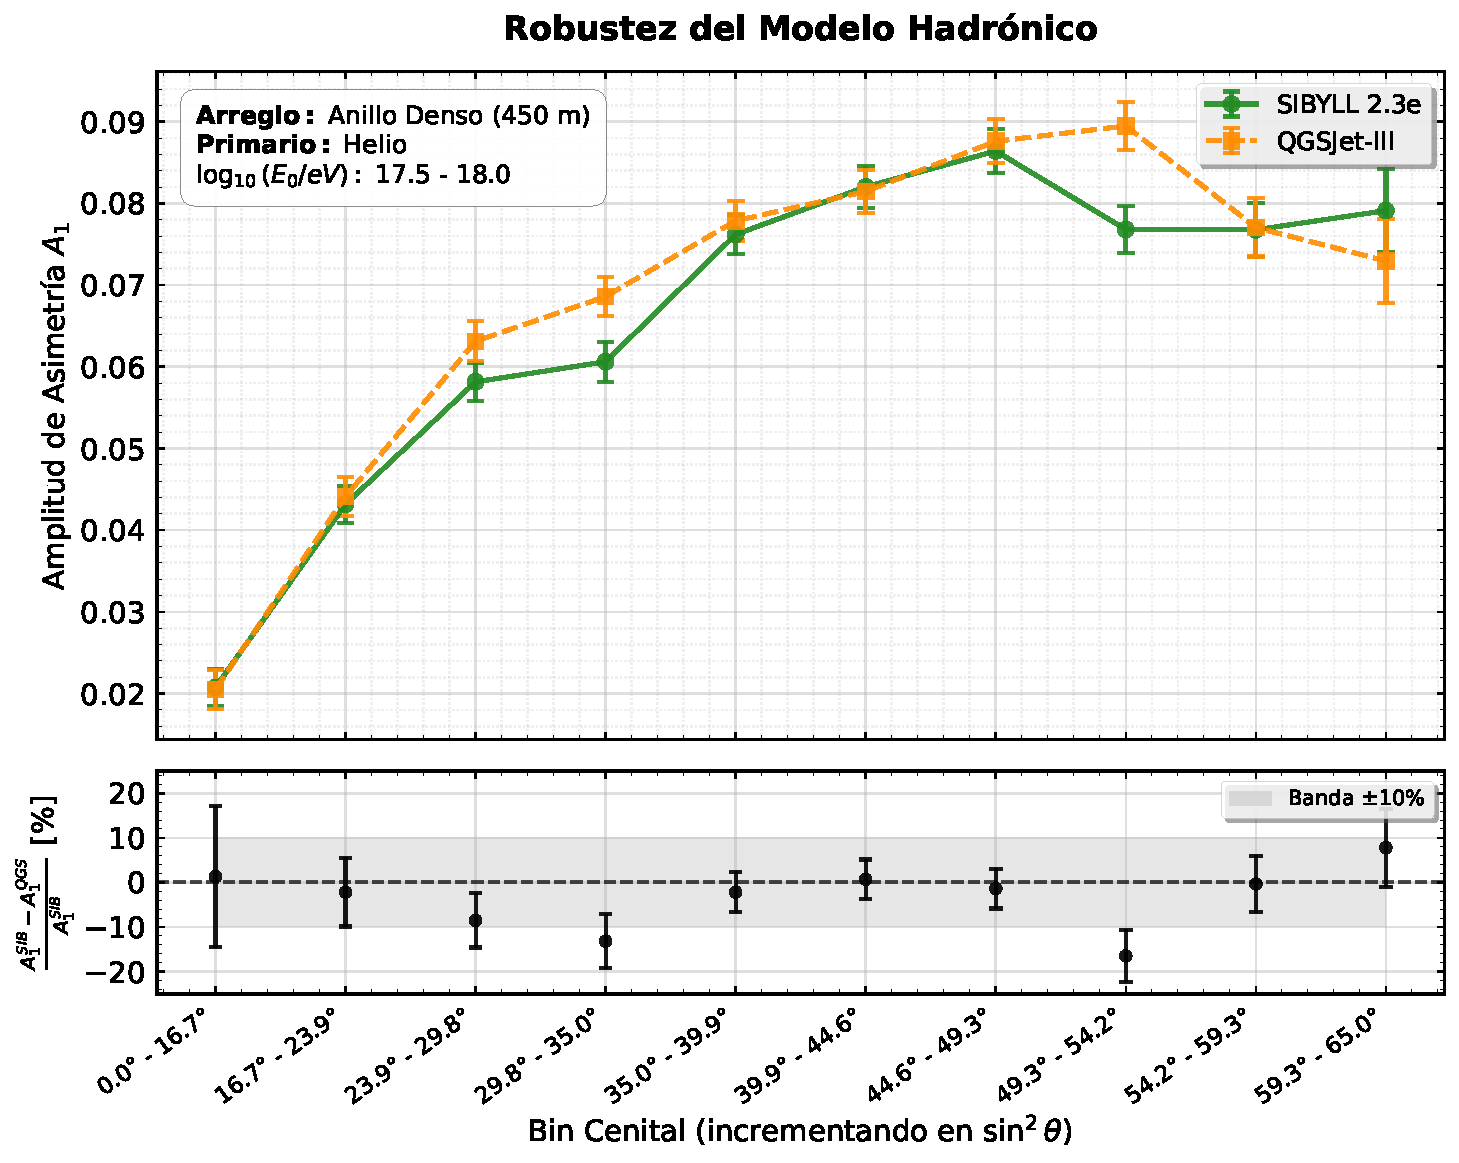
\includegraphics[width=1\textwidth]{capitulos/imagenes_capitulos/cap5/Hadronic_Uncertainty_Helium.pdf}
	\caption{Comparación de la amplitud $A_1$ para lluvias de helio simuladas con diferentes modelos hadrónicos. El panel inferior muestra sus diferencias relativas. La semejanza de tendencias describe esta muestra y no establece independencia universal del modelo.}
	\label{fig:modelos_hadronicos}
\end{figure}

En la comparación presentada, ambos modelos muestran una evolución angular semejante. Las diferencias relativas se encuentran mayormente dentro de la banda del $\pm10\%$ indicada en la figura, con desviaciones puntuales del orden del $15\%$. Estos valores describen el control realizado para helio y no establecen independencia universal del modelo. Cerca de amplitudes pequeñas, las diferencias absolutas y sus incertidumbres resultan más informativas que un cociente relativo. Combinar muestras de distintos modelos requiere justificar previamente el propósito y la ponderación.

\subsection{Dependencia de la amplitud $A_1$ con la energía del primario}
\label{subsec:dependencia_energia}

Para evaluar la estabilidad del observable frente a variaciones cinemáticas, se analizó la evolución del parámetro de asimetría $A_1$ en función de la energía del rayo cósmico primario dentro de la banda de interés, $\log_{10}(E/\mathrm{eV}) \in [17.5, 18.0]$. Utilizando el conjunto de simulaciones de protones (\texttt{SIBYLL 2.3e}) restringido al rango angular de mayor desarrollo de asimetría ($40^\circ \leq \theta \leq 60^\circ$), los datos se particionaron en 5 bines de energía reconstruida. Los resultados de los ajustes armónicos para cada intervalo se presentan en la Figura \ref{fig:a1_vs_energia}.

\begin{figure}[H]
	\centering
	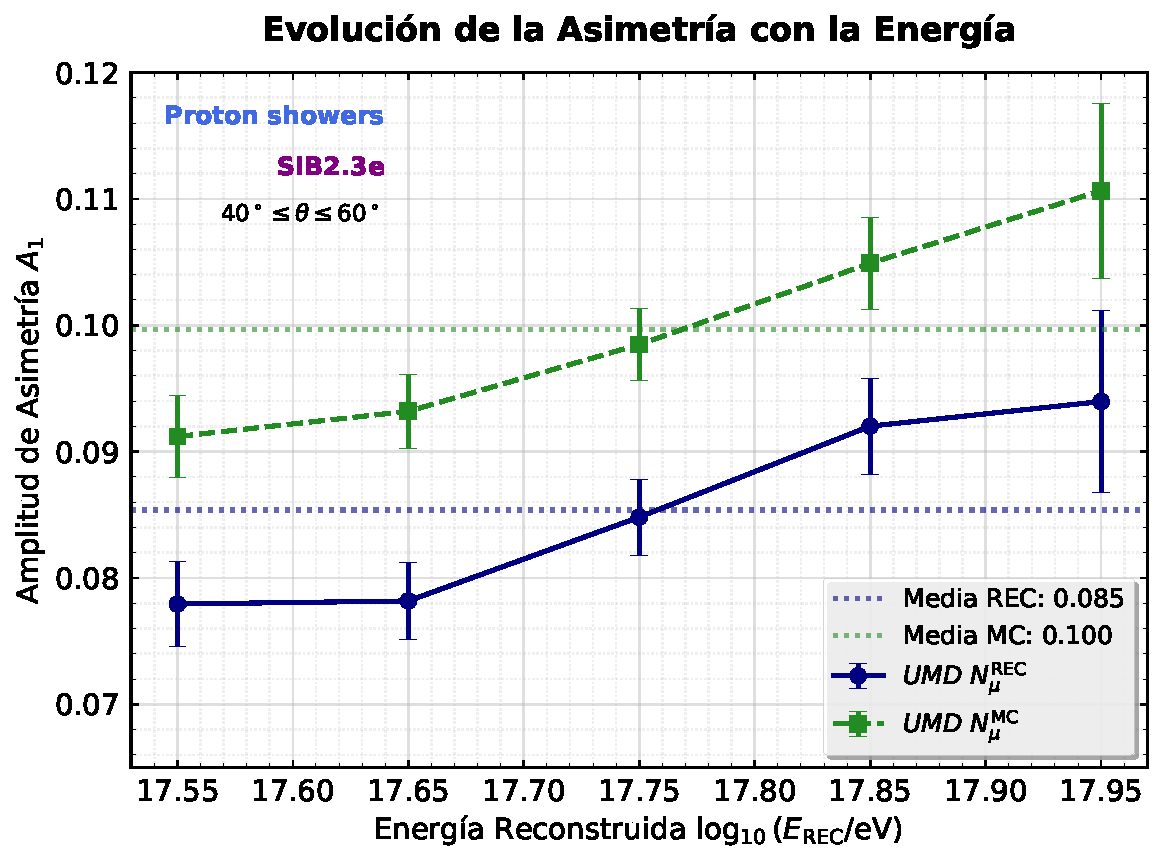
\includegraphics[width=1\textwidth]{capitulos/imagenes_capitulos/cap5/DenseRing_Systematics_Energy.pdf}
	\caption{Evolución de la amplitud de asimetría $A_1$ en función de la energía reconstruida para cascadas de protón simuladas con \texttt{SIBYLL 2.3e}. Se observa un leve incremento lineal en la asimetría a mayores energías, presente tanto a nivel Monte Carlo como en la reconstrucción.}
	\label{fig:a1_vs_energia}
\end{figure}

A priori, al tratarse de un rango energético relativamente estrecho (media década logarítmica), no se esperaba observar una fuerte dependencia funcional. Sin embargo, los resultados revelan un leve pero sistemático incremento lineal de la amplitud $A_1$ a medida que aumenta la energía, comportamiento que es capturado consistentemente tanto por los datos ideales (MC) como por los reconstruidos (REC).

Una hipótesis interpretativa vincula el crecimiento con cambios en la distribución longitudinal de producción de muones. Si la contribución dominante proviniera de una región más próxima al suelo, aumentaría la escala geométrica $r\tan\theta/D$. Sin embargo, también cambiarían la pendiente angular y los pesos de supervivencia. Además, $X_{\mathrm{max}}$ electromagnético y el perfil de producción muónica no son intercambiables. La dependencia con energía observada no demuestra por sí sola una relación causal con un único máximo longitudinal ni una ley universal $A_1\propto1/D$.

La variación absoluta reportada en esta media década es del orden de $\Delta A_1\approx0.015$. Integrar el intervalo aumenta la estadística, pero esa escala no garantiza por sí sola ausencia de sesgos de mezcla. Para comparar primarios deben controlarse sus distribuciones de energía y cenital, ya que una correlación entre estas variables y el azimut puede modificar el coeficiente integrado.

\subsection{Discriminación de Masa Primaria: Protón vs. Hierro}
\label{sec:discriminacion_masa}

Habiendo caracterizado la modulación y sus controles de reconstrucción en el entorno del Anillo Denso, el objetivo culminante de este análisis es evaluar la capacidad del observable $A_1$ para discriminar la naturaleza química del rayo cósmico primario. Para ello, se compararon las distribuciones de amplitud de asimetría para las poblaciones extremas de masa: primarios livianos (protones) y primarios pesados (hierro, con número másico $A=56$). 

Al evaluar el parámetro $A_1$ para ambos conjuntos de datos con energías $\log_{10}(E/\mathrm{eV}) \in [17.5, 18.0]$ usando el modelo hadrónico \texttt{Sibyll 2.3e}, se observó una separación sistemática entre las curvas. La población de protones desarrolla amplitudes de asimetría consistentemente mayores a las correspondientes a la población de hierro a lo largo del rango angular evaluado para la mayoría de los bines.

\subsubsection{El Factor de Mérito ($MF$) y el \textit{Sweet Spot} de discriminación}
\label{subsec:sweet_spot}

La comparación utiliza el cociente denominado $MF$ en la figura:
\begin{equation}
MF=\frac{|\widehat A_1^{\mathrm P}-\widehat A_1^{\mathrm{Fe}}|}
{\sqrt{\sigma_{\widehat A_1^{\mathrm P}}^2+\sigma_{\widehat A_1^{\mathrm{Fe}}}^2}}.
\end{equation}
En el procedimiento que genera esta figura, las cantidades del denominador son incertidumbres de los ajustes de las muestras, no anchos intrínsecos de distribuciones de $A_1$ por lluvia. Por ello, el cociente describe separación entre estimaciones para dos muestras, bajo el modelo de errores utilizado y sin covarianza entre ellas. No mide directamente capacidad de clasificar la masa de una lluvia individual.

Este estudio corresponde al muestreo idealizado del Anillo Denso; no constituye una prestación alcanzada por el arreglo real ni una cota superior matemática de su sensibilidad. La Figura~\ref{fig:mf_sweet_spot} muestra una ventana favorable alrededor de $40^\circ$--$55^\circ$, con valores reportados del orden de $2.5$. La interpretación como significancia requiere validar las incertidumbres, incluyendo la reutilización de lluvias y las correlaciones entre estaciones; tampoco corresponde interpretar el máximo explorado como una significancia global.

\begin{figure}[H]
	\centering
	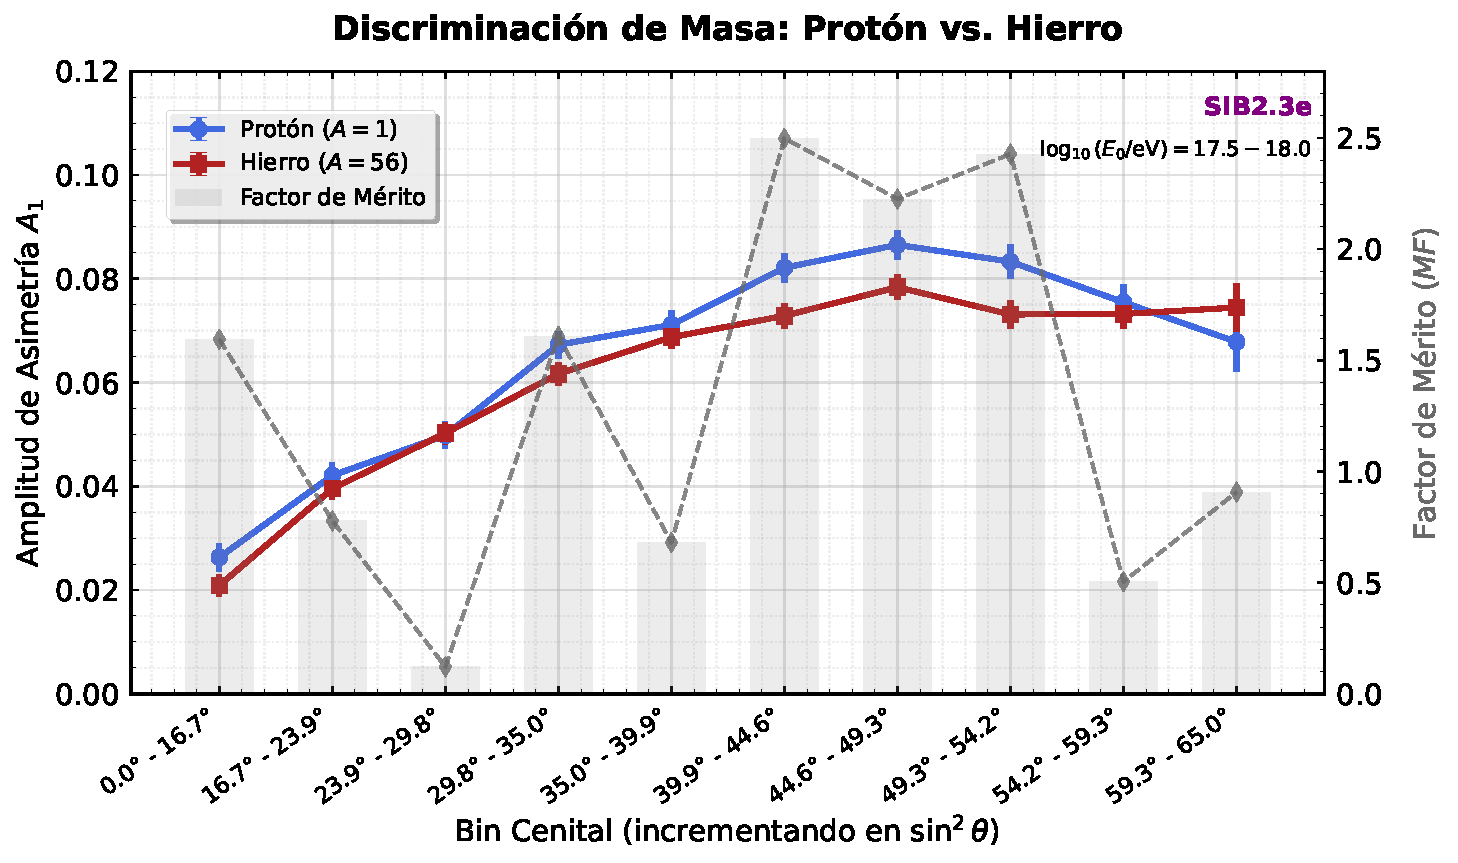
\includegraphics[width=1\textwidth]{capitulos/imagenes_capitulos/cap5/Mass_Discrimination_MF.pdf}
	\caption{Evolución del Factor de Mérito ($MF$) en función del ángulo cenital. Se observa una ventana de mayor separación entre las amplitudes ajustadas alrededor de $40^\circ$--$55^\circ$. El cociente utiliza errores de los ajustes, no dispersión evento a evento.}
	\label{fig:mf_sweet_spot}
\end{figure}

A bajas inclinaciones la componente temprano--tardía es pequeña y su diferencia entre primarios resulta más difícil de resolver. A inclinaciones altas intervienen simultáneamente la respuesta instrumental, la selección y la estadística disponible. La degradación del cociente no permite asignar exclusivamente la causa a un corrimiento del núcleo. Estos resultados motivan estudiar sensibilidad a composición a nivel de poblaciones, sin equipararla todavía a discriminación evento a evento.

\subsection{Interpretación física y desarrollo longitudinal}
\label{subsec:interpretacion_fisica}

La tendencia $\widehat A_1^{\mathrm P}>\widehat A_1^{\mathrm{Fe}}$ constituye un resultado de las muestras estudiadas. Una conexión con el desarrollo longitudinal es físicamente plausible, pero no equivale a medir una relación única $A_1(X_{\mathrm{max}})$. En el modelo de superposición, un primario de número másico $A$ y energía $E_0$ se aproxima por subcascadas nucleónicas de energía $E_0/A$ \cite{matthews2005}. Las simulaciones predicen, en promedio, un máximo más alto para primarios pesados. Las mediciones de fluorescencia y su comparación con modelos proporcionan el contexto de la Figura~\ref{fig:auger_xmax}; no son observaciones de primarios etiquetados individualmente como protón o hierro.

\begin{figure}[H]
	\centering
	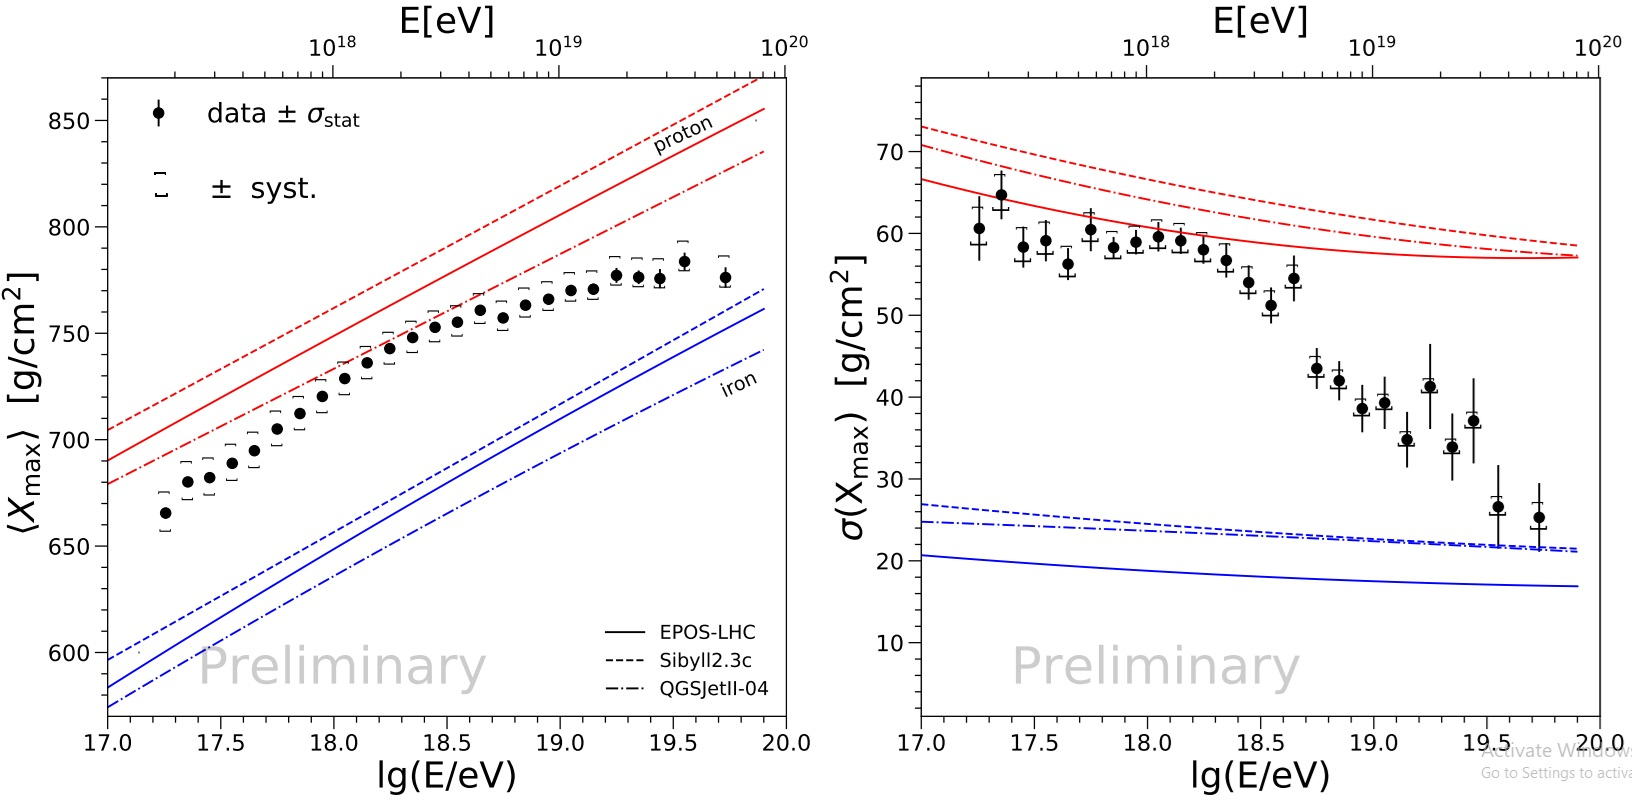
\includegraphics[width=1\textwidth]{capitulos/imagenes_capitulos/cap5/x_max.jpg}
	\caption{Evolución del valor medio de $X_{\text{max}}$ (izquierda) y sus fluctuaciones (derecha) en función de la energía primaria, medido por el Observatorio Pierre Auger. Se observan las curvas teóricas de los modelos hadrónicos acotando el comportamiento entre protón (líneas rojas superiores) y hierro (líneas azules inferiores). La comparación con curvas de primarios es dependiente del modelo hadrónico. Extraído de \cite{yushkov2019mass}.}
	\label{fig:auger_xmax}
\end{figure}

El perfil de la Figura~\ref{fig:longitudinal_profile} ilustra el crecimiento y decrecimiento de una cascada. La producción de muones tiene su propio perfil y máximo $X_{\mathrm{max}}^\mu$, determinados por la cascada hadrónica y el decaimiento de mesones \cite{Cazon2012}. No se supone que este máximo coincida con el electromagnético.

\begin{figure}[H]
	\centering
	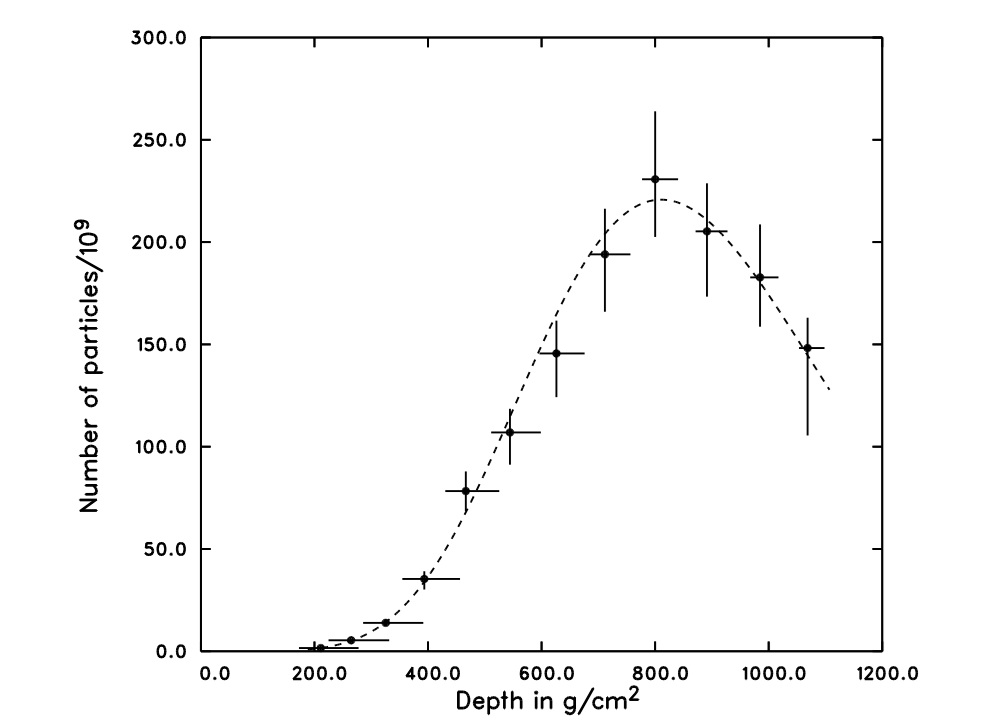
\includegraphics[width=1\textwidth]{capitulos/imagenes_capitulos/cap5/ammount_xmax.jpg}
	\caption{El gráfico corresponde al evento de mayor energía detectado por el experimento Fly's Eye ($E \approx 3.2 \times 10^{20}$ eV) extraído de \cite{FlysEye1995}. Se observa claramente la fase de multiplicación hasta alcanzar la profundidad del máximo, seguida de la atenuación de la cascada. $X_{\mathrm{max}}$ es una profundidad atmosférica, expresada en masa por unidad de área, no una distancia geométrica.}
	\label{fig:longitudinal_profile}
\end{figure}

Para una fuente axial ilustrativa, la Ec.~\ref{eq:geometria_fuente_muonica} introduce la escala $r\tan\theta/D$. Si se conservara únicamente la dilución $1/L^2$, con $r\ll D$ y $r\tan\theta\ll D$, su primer armónico sería
\begin{equation}
A_{1,\mathrm{dil}}\simeq2\frac{r}{D}\tan\theta.
\label{eq:asym_mu_cinematica}
\end{equation}
El uso de $\tan\theta$, y no $\sin\theta$, corresponde a mantener fijo el radio en el plano de la lluvia. Ésta es la contribución de dilución, no una fórmula completa para $A_1^\mu$: omite la distribución angular, la supervivencia, la apertura y la selección. Una menor distancia de producción aumenta este término positivo, pero también modifica los otros. Por ello no se utiliza como demostración cuantitativa de la dependencia de masa o energía.

Un contraste decisivo requeriría estudiar conjuntamente el perfil de producción muónica, la distribución de energías que alcanza cada radio y la respuesta del UMD. Las tendencias observadas motivan esa conexión longitudinal; no justifican atribuir todo el efecto a atenuación ni, alternativamente, a una proyección pura.

\subsubsection{Contraste fenomenológico con el Detector de Superficie}
\label{subsec:contraste_sd_bradfield}

Los estudios del SD \cite{BradfieldThesis} muestran que la interpretación de su asimetría depende de la composición de la señal y del estado de desarrollo. Un argumento local para una componente electromagnética en atenuación puede escribirse definiendo $X(\phi)=X_0-\Delta X_1\cos\phi$, con $\Delta X_1>0$:
\begin{equation}
A_{1,\mathrm{EM}}\simeq-\Delta X_1
\left.\frac{\partial\ln S_{\mathrm{EM}}}{\partial X}\right|_{X_0}.
\label{eq:asym_em_taylor}
\end{equation}
Si la derivada es negativa, el resultado es positivo: exceso temprano. La aproximación mantiene fijas las demás dependencias y no incorpora por separado todo el transporte transversal \cite{dova2003}. Una pendiente más suave cerca del máximo puede reducir esta contribución. No establece una relación universal entre $X_{\mathrm{max}}$ y la asimetría total del SD.

Si las componentes de señal están definidas para una misma muestra y admiten la misma descripción armónica, la suma lineal da
\begin{equation}
A_1^{\mathrm{SD}}=
f_\mu^S A_{1,\mu}^S+f_{\mathrm{EM}}^S A_{1,\mathrm{EM}}^S,
\qquad
f_j^S=\frac{S_{0,j}}{S_{0,\mu}+S_{0,\mathrm{EM}}}.
\end{equation}
Se trata de fracciones de \emph{señal}, no de número de partículas. Aumentar el contenido muónico puede reducir la asimetría total si la señal muónica es menos asimétrica que la electromagnética; no modifica necesariamente la asimetría relativa de los propios muones. El coeficiente de conteos SD-Muon(MC) no puede sustituirse sin más por $A_{1,\mu}^S$.

\paragraph{Qué se cancela en el tanque.}
La contribución de la geometría del recipiente debe distinguirse de la asimetría del flujo incidente. Para una dirección fija y un haz localmente uniforme de muones atravesantes, el área proyectada $\mathcal A_\perp$ y la cuerda media $\langle\ell\rangle$ de un volumen convexo satisfacen
\begin{equation}
\mathcal A_\perp(\vartheta)\langle\ell(\vartheta)\rangle=V,
\qquad
S_\mu\propto F_\perp(\phi)V.
\label{eq:dense2026_tanque}
\end{equation}
Si la señal es proporcional al recorrido en agua, la mayor señal media por trayectoria compensa exactamente el cambio de apertura. La cancelación es local, dirección por dirección y en cada región de la lluvia; no requiere que $F_\perp$ sea igual en la zona temprana y en la tardía \cite{GAP2000_017}. Por ello, el recorrido más largo de ciertas trayectorias no constituye por sí solo una nueva contribución negativa al armónico de la señal muónica.

El resultado se refiere a una respuesta ideal lineal con muones atravesantes: trayectorias que se detienen, umbrales y respuesta óptica no uniforme exigen su propio tratamiento. Tampoco anula la asimetría del flujo $F_\perp$ ni la apertura de un conteo de partículas, para el cual $N_\mu\propto F_\perp\mathcal A_\perp$ sin ponderar por $\ell$. Finalmente, la identidad no corrige una selección de estaciones basada en la señal total. Éstas son limitaciones del observable, no excepciones al balance geométrico ideal.

El UMD reduce la mezcla electromagnética y estudia una población muónica filtrada por el suelo, pero conserva sensibilidad a geometría, energía y selección. Esta complementariedad permite investigar la cascada con observables distintos. La inversión del conteo seleccionado del SD en el Infill exige además el control de selección del capítulo siguiente y no valida retrospectivamente una explicación por muones blandos del Anillo Denso.

\subsection{Balance del estudio del Anillo Denso}
\label{subsec:dense2026_balance}

El anillo establece una modulación muónica positiva en las muestras estudiadas, una diferencia entre conteos MC y REC y tendencias con energía, inclinación y primario. La regularidad espacial permite estudiar esos efectos con mayor control que en el arreglo real. El remuestreo direccional muestra que la dependencia azimutal de los errores de conteo puede reducir la amplitud; el patrón del error radial señala, por separado, una distorsión geométrica alineada con el eje temprano--tardío.

La interpretación debe conservar esas distinciones. Ni el signo positivo del UMD demuestra dominancia exclusiva de atenuación, ni la compensación de apertura y cuerda del tanque elimina los efectos de selección. El control del capítulo siguiente demuestra una inversión inducida por \texttt{HasStation} para el conteo muónico SD en la muestra \textit{Infill} ensayada. Ese resultado cambia la interpretación de dicha inversión, pero no constituye una corrección cuantitativa de las curvas del Anillo Denso. En consecuencia, la sensibilidad a masa presentada aquí es un resultado de simulación bajo su geometría y selección específicas; su transferencia al arreglo real exige controlar conjuntamente selección, conteo y reconstrucción geométrica.

\newpage

\clearpage
% !TEX root = vista_previa.tex
% BORRADOR INTEGRADO, 24-09-2026. No reemplaza el capitulo autorizado.
% Procedencia y limites de los resultados: 06_NOTAS.md.

\section{Dinámica radial y selección de estaciones en el arreglo \textit{Infill}}
\label{cap:infill}

El estudio del Anillo Denso se extiende a la geometría del arreglo \textit{Infill}, con separación nominal de $750$~m entre estaciones. A diferencia de la configuración de radio fijo, este arreglo permite examinar la evolución de la asimetría en función de la distancia al eje, empleando las posiciones de los tanques de superficie y de los módulos enterrados. La muestra principal corresponde a protones simulados con \texttt{SIBYLL 2.3e}, en el intervalo $17.5\leq\log_{10}(E_0/\mathrm{eV})<18.0$.

Se distinguen tres operaciones que pueden modificar el observable: seleccionar las estaciones que participan del promedio, reconstruir su conteo o señal y reconstruir las coordenadas de la lluvia. Utilizar núcleo y dirección Monte Carlo elimina el error de esas coordenadas, pero no elimina una selección de estaciones realizada previamente. Esta distinción permite interpretar la inversión del coeficiente muónico del SD sin atribuirla a una inversión de la densidad muónica no seleccionada.

En todo el capítulo se conserva la convención $\phi=0$ para la región temprana y $\phi=\pm\pi$ para la tardía. Por lo tanto, $A_1>0$ indica exceso temprano y $A_1<0$, exceso tardío. El radio $r$ es la distancia al eje en el plano perpendicular a la dirección de la lluvia.

\subsection{Evolución radial con geometría Monte Carlo}
\label{subsec:infill_mc}

Se calculan inicialmente las coordenadas de cada estación utilizando el núcleo y los ángulos verdaderos. Para limitar la mezcla de densidades dentro de cada intervalo se excluye $r<150$~m y se utilizan coronas de referencia de $150$~m, con las adaptaciones estadísticas de las figuras originales. El corte cercano al núcleo se motiva por el fuerte gradiente de la distribución lateral y la sensibilidad a cambios de posición; no presupone una divergencia angular extrema en esa región. El azimut se divide en doce intervalos de $30^\circ$ y la inclinación en bandas de referencia de $10^\circ$, con una banda final $50^\circ\leq\theta<65^\circ$.

Los perfiles se ajustan con el primer armónico de la Ec.~\ref{eq:ajuste_armonico}. Las grillas completas se presentan en el Anexo~\ref{anexo:ajustes_infill_mc}. Un valor de $\chi^2/\mathrm{ndf}$ cercano a la unidad indica compatibilidad con esa parametrización bajo las incertidumbres utilizadas; no demuestra que los armónicos superiores sean exactamente nulos. Asimismo, una amplitud no significativa no debe confundirse con ausencia física de asimetría.

\begin{figure}[H]
\centering
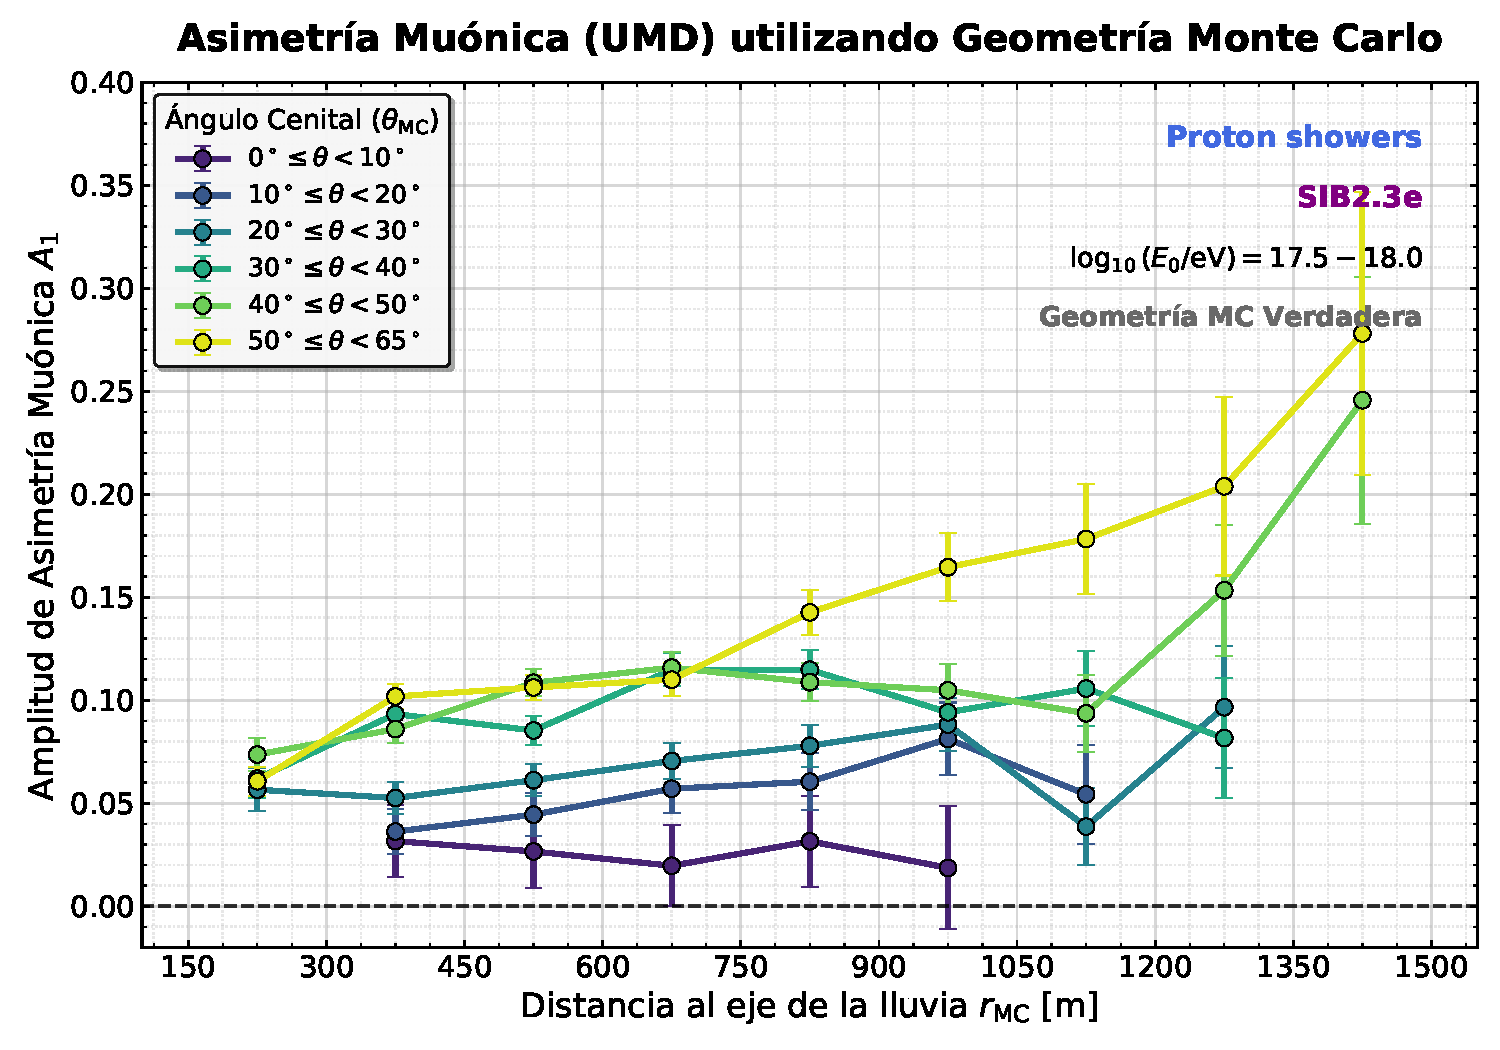
\includegraphics[width=\textwidth]{capitulos/imagenes_capitulos/cap6/Global_A1_vs_R_Theta_MC.pdf}
\caption{Evolución radial de $A_1$ en el UMD para distintas inclinaciones, con geometría Monte Carlo. Se conservan las condiciones de selección de la muestra original. Los intervalos mostrados no constituyen una medición de una población UMD previa a toda selección instrumental.}
\label{fig:a1_vs_r_theta_mc}
\end{figure}

La Figura~\ref{fig:a1_vs_r_theta_mc} muestra una modulación pequeña para lluvias cuasi-verticales y valores predominantemente positivos al aumentar la inclinación. En bandas intermedias aparecen cambios de pendiente y una posible estabilización radial; en las más inclinadas, el crecimiento es más marcado. Estas tendencias caracterizan el observable seleccionado. Su signo positivo es compatible tanto con proyección geométrica como con supervivencia diferencial y con la competencia cinemática discutida en el capítulo~3; no permite identificar por sí solo cuál domina. Las estructuras puntuales deben evaluarse teniendo en cuenta las fluctuaciones entre lluvias y la mezcla de energía, inclinación y radio dentro de cada intervalo.

Para separar la respuesta del conteo de los errores de coordenadas se comparan $N_\mu^{\mathrm{MC}}$ y $N_\mu^{\mathrm{REC}}$ manteniendo fija la geometría Monte Carlo. En la banda $40^\circ\leq\theta<50^\circ$, la Figura~\ref{fig:umd_rec_vs_mc_theta} conserva la tendencia radial general y muestra una modificación de amplitud. El estudio del sesgo direccional del conteo en el Anillo Denso ofrece un antecedente para interpretar esta diferencia, pero no sustituye una validación específica del Infill.

\begin{figure}[H]
\centering
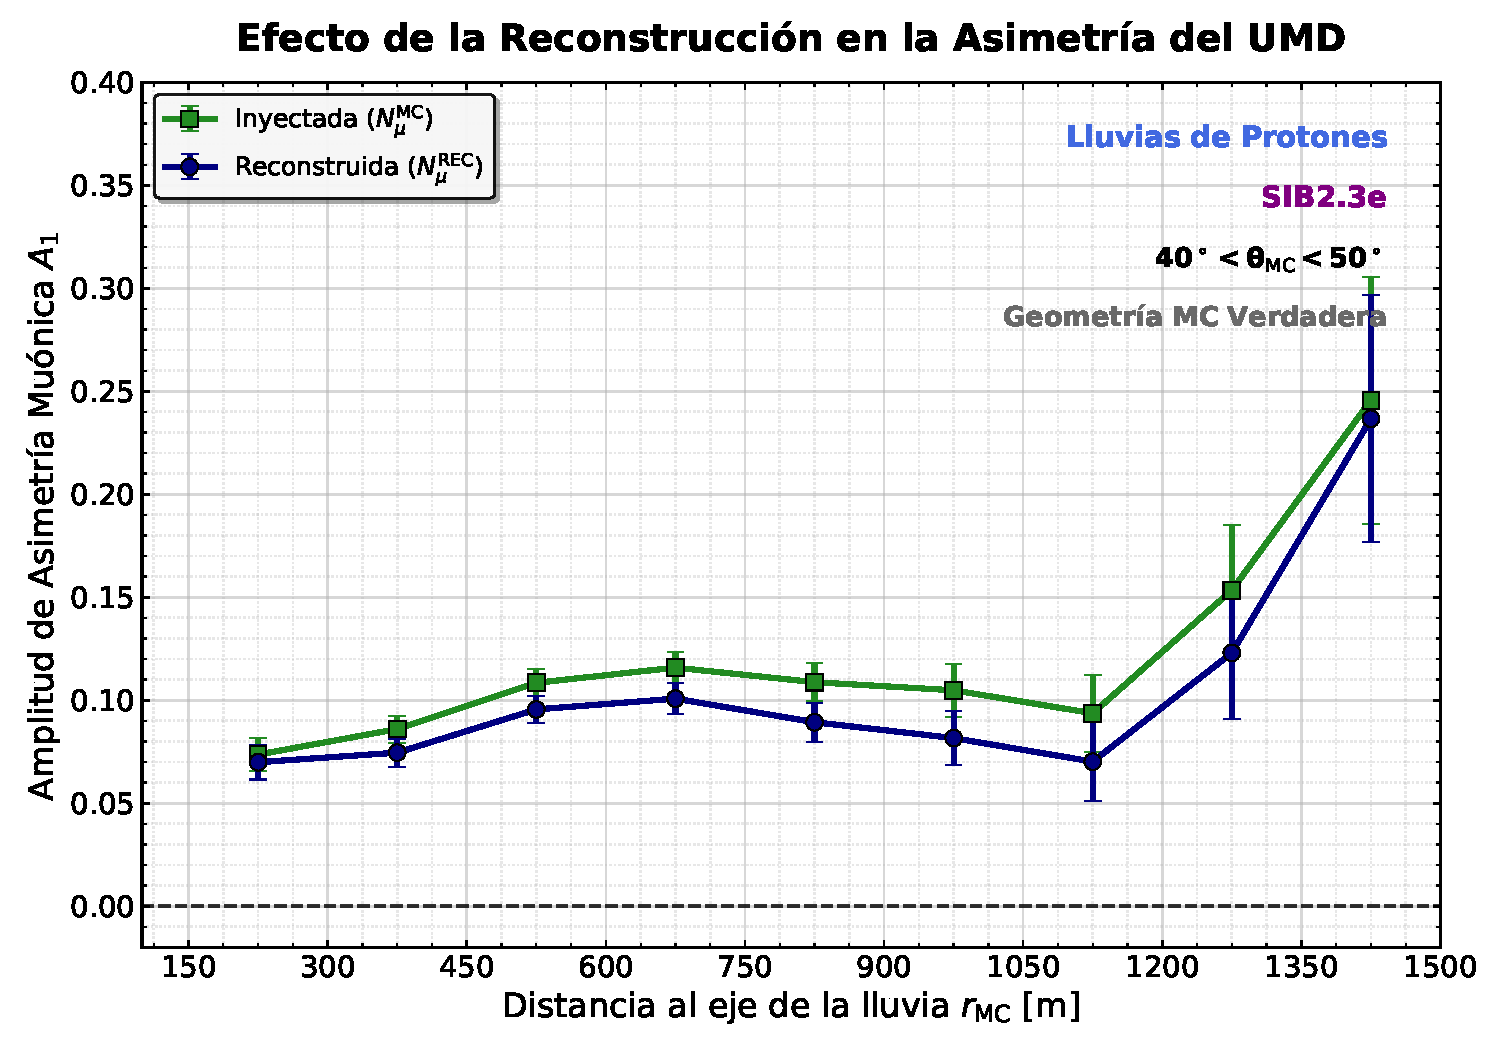
\includegraphics[width=\textwidth]{capitulos/imagenes_capitulos/cap6/UMD_Asymmetry_MC_vs_REC.pdf}
\caption{Comparación del número de muones Monte Carlo y reconstruido para $40^\circ\leq\theta<50^\circ$, manteniendo núcleo y dirección Monte Carlo. Se examina el cambio de conteo dentro de la muestra seleccionada, no el efecto de cambiar las coordenadas de las estaciones.}
\label{fig:umd_rec_vs_mc_theta}
\end{figure}

\subsubsection{UMD y señal total del SD}
\label{subsubsec:umd_vs_sd_mc}

El UMD proporciona un conteo de muones que atravesaron el suelo, mientras que SD Total es una señal reconstruida y calibrada en VEM. Las diferencias entre ambos incluyen transporte, área sensible, respuesta y selección. Mantener las coordenadas verdaderas controla únicamente la parte geométrica de la reconstrucción de la lluvia.

En la Figura~\ref{fig:umd_vs_sd_mc}, para $30^\circ\leq\theta<40^\circ$, el UMD conserva una asimetría predominantemente positiva, mientras que la señal SD disminuye y alcanza valores negativos a grandes distancias. Cerca del radio del Anillo Denso se recupera un comportamiento cualitativamente comparable al de aquella configuración. La inversión lejana es un resultado del observable medido en la muestra retenida, no una demostración de que el flujo muónico incidente sobre toda estación simulada tenga exceso tardío.

\begin{figure}[H]
\centering
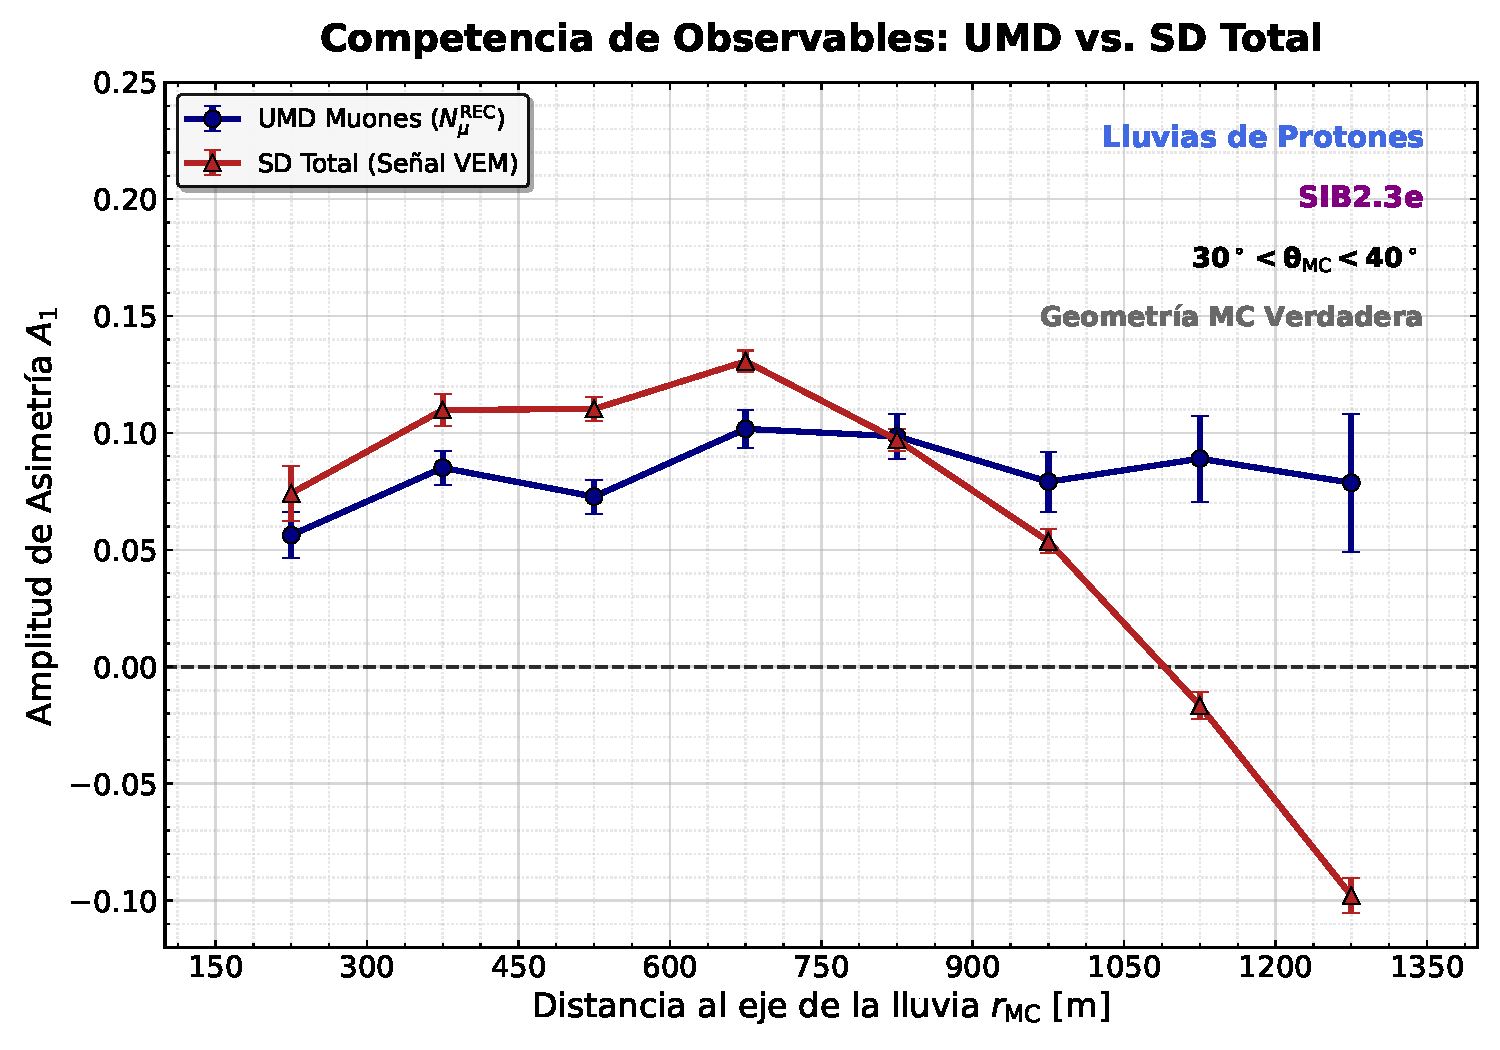
\includegraphics[width=\textwidth]{capitulos/imagenes_capitulos/cap6/UMD_vs_SD_Total_Asymmetry.pdf}
\caption{UMD frente a señal total SD para $30^\circ\leq\theta<40^\circ$, utilizando geometría Monte Carlo. La inversión de la señal SD se observa dentro de la selección original de estaciones. Los dos detectores no miden la misma población ni la misma magnitud física.}
\label{fig:umd_vs_sd_mc}
\end{figure}

\subsubsection{Conteos muónicos y electromagnéticos del SD}
\label{subsubsec:desglose_sd}

La simulación permite estudiar por separado los conteos de muones y de electrones más fotones asociados al SD. Estos conteos de partículas no son componentes de la señal expresadas en VEM: su suma no reconstruye SD Total, porque la respuesta depende de la especie, la energía y la trayectoria.

En la Figura~\ref{fig:desglose_sd_mc}, el coeficiente electromagnético permanece positivo y el muónico del SD cambia de signo en la periferia. La inversión aparece, por tanto, incluso en una cantidad etiquetada como verdad Monte Carlo. Sin embargo, la condición de verdad se refiere al valor del conteo, no a la ausencia de selección de las estaciones donde se consulta.

\begin{figure}[H]
\centering
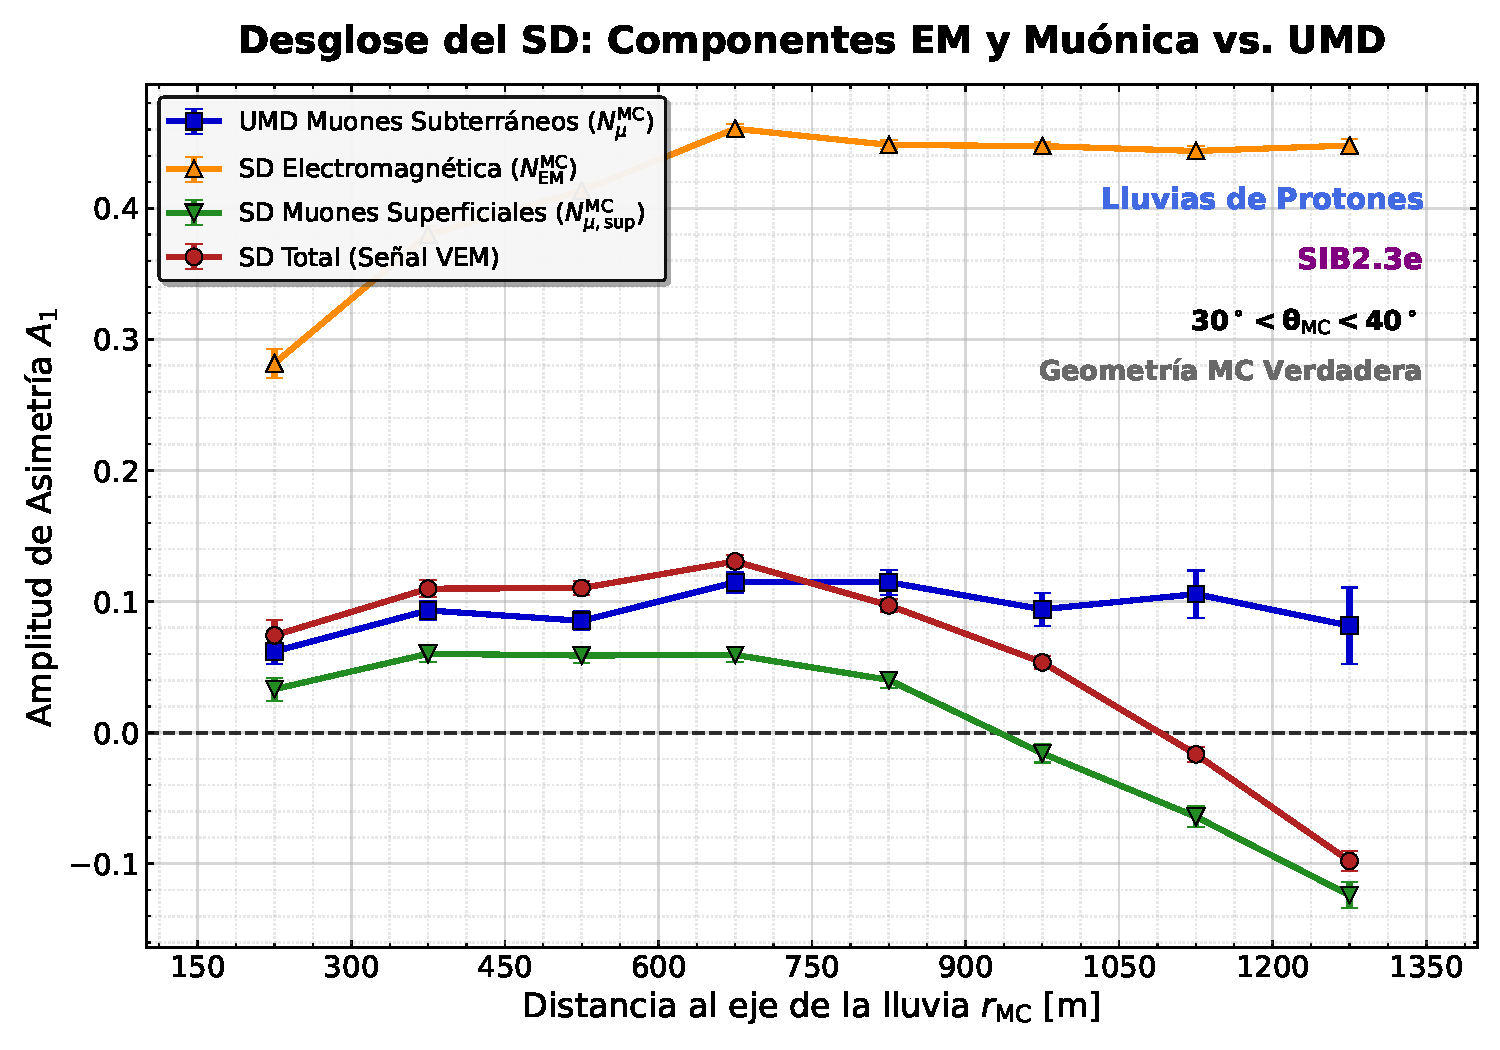
\includegraphics[width=\textwidth]{capitulos/imagenes_capitulos/cap6/SD_Desglose_Componentes_vs_UMD.pdf}
\caption{Coeficientes de los conteos muónico y electromagnético Monte Carlo del SD, del UMD y de la señal total reconstruida, para $30^\circ\leq\theta<40^\circ$. El SD muónico negativo corresponde a la muestra seleccionada por el procesamiento. La figura no identifica por sí sola un mecanismo de propagación responsable de ese signo.}
\label{fig:desglose_sd_mc}
\end{figure}

La explicación de esta inversión por una proyección necesariamente negativa de muones blandos no se sostiene: para el flujo radial saliente y descendente, $\langle p_r/(-p_z)\rangle\tan\theta$ es positivo. La preferencia angular por la región tardía es un efecto diferente, que compite con la dilución espacial y la supervivencia. El modelo analítico de producción y transporte permite estudiar esa competencia \cite{Cazon2012,Luce_ICRC2021}, pero su evaluación simplificada no justificaba el signo negativo del conteo seleccionado. Tampoco el umbral del UMD equivale al límite de momento longitudinal infinito ni anula su proyección geométrica.

La explicación por mayor recorrido en el agua debe distinguirse de la anterior. Para muones pasantes, respuesta proporcional a longitud recorrida y flujo aproximadamente uniforme sobre el tamaño del tanque, se cumple $A_\perp\langle\ell\rangle=V$. La menor o mayor apertura se compensa con la longitud media de cuerda, para cada dirección y en cada región. El término geométrico adicional así obtenido es nulo en la señal muónica ideal: no es una contribución tardía negativa. Esta cancelación no anula la asimetría del flujo incidente, no se aplica al conteo puro y no garantiza una respuesta nula de un tanque real con disparo y selección. La inversión de la Figura~\ref{fig:desglose_sd_mc} exige, por tanto, examinar la definición completa de la muestra.

\subsection{La inversión del SD como efecto de selección}
\label{subsec:control_seleccion_sd}

\subsubsection{Del conteo verdadero al promedio condicionado}

El procesamiento original recorría los contadores UMD y exigía que existiera una estación SD reconstruida asociada mediante \texttt{HasStation(sdId)}. Sólo después recuperaba el conteo SD de verdad Monte Carlo, \texttt{GetNumberOfMuons()}. Esa condición no cambia cuántos muones tiene una estación retenida, pero sí determina cuáles estaciones aportan al promedio azimutal.

La auditoría de la implementación local de simulación identifica este conteo como un contador de candidatos muónicos cuya trayectoria intercepta geométricamente el volumen de agua, previo a la propagación detallada en Geant4. No es una estimación de muones obtenida dividiendo una señal Cherenkov, ni se incrementa mediante un umbral óptico. La respuesta del agua sí puede intervenir en la presencia de una estación reconstruida. Es posible, entonces, contar correctamente los muones y obtener una media sesgada respecto de la población anterior a esa condición.

Sea $I$ el indicador de presencia de estación reconstruida, con $I=1$ cuando \texttt{HasStation} es verdadero. Dentro de una misma banda de radio, inclinación y energía, la identidad
\begin{equation}
\left\langle N_\mu\mid\phi,I=1\right\rangle
=\left\langle N_\mu\mid\phi\right\rangle
+\frac{\operatorname{Cov}(N_\mu,I\mid\phi)}{P(I=1\mid\phi)}
\label{eq:infill2026_media_condicionada}
\end{equation}
vale cuando $P(I=1\mid\phi)>0$. Expresa exactamente qué cambia: el promedio de la población retenida incluye la correlación del conteo con la selección. Si esa contribución relativa es mayor en la región tardía, puede invertir el coeficiente del promedio seleccionado aunque el anterior a la selección sea positivo. No se han creado ni desplazado muones.

Una exposición azimutal desigual no es equivalente a este efecto. Si $I$ fuera independiente del conteo a $\phi$ fijo, el término de covarianza sería cero: reducir la cantidad de estaciones aumentaría la incertidumbre sin cambiar sistemáticamente la media. La comparación pertinente debe variar la condición de selección sobre las mismas estaciones simuladas y los mismos eventos disponibles.

\subsubsection{Control con los ADST y reproducción del procesamiento}

Los ADST conservan una colección de estaciones SD simuladas que puede leerse aunque no exista su contraparte reconstruida. El control recorre esa colección de forma independiente de los módulos UMD, guarda el indicador $I$ y cuenta una sola vez cada combinación de archivo, evento y estación SD. La extracción por módulos se conserva separadamente para reproducir el análisis UMD original. No basta con quitar un filtro dentro del recorrido UMD: una estación que no aparece en ese recorrido seguiría ausente del conjunto SD.

Se utilizaron veinte archivos de protones \texttt{SIBYLL 2.3e} del intervalo energético ya indicado. En la selección de estaciones físicas del Infill, $30^\circ\leq\theta<40^\circ$ y $150\leq r<1800$~m, se dispone de $106280$ registros estación--evento SD: $51031$ con $I=1$ y $55249$ con $I=0$. ``Antes'' designa todas las estaciones simuladas disponibles en esos ADST; no todos los eventos de CORSIKA originalmente generados ni una muestra previa a todas las selecciones de escritura.

La verificación del reprocesamiento contra la tabla anterior conserva los $1589487$ registros originales de módulos y sus columnas originales. Este control de preservación es distinto del número de estaciones SD recuperadas: las filas de módulos no constituyen el denominador del promedio por estación SD. Además, los conteos y coordenadas del SD seleccionado coinciden con la referencia anterior para las mismas claves de estación y evento.

Para reproducir la comparación radial se mantienen ocho intervalos de $150$~m entre $150$ y $1350$~m y doce intervalos azimutales. En cada corona se normalizan las medias azimutales por su media y se ajusta $1+A_1\cos\phi$, ponderando por los errores estándar de esas medias. Se aplica exactamente el mismo estimador antes y después de \texttt{HasStation}. La reproducción del nuevo conjunto de datos recupera los coeficientes, errores formales y tamaños de muestra de los ajustes de referencia muónicos y electromagnéticos.

\begin{figure}[H]
\centering
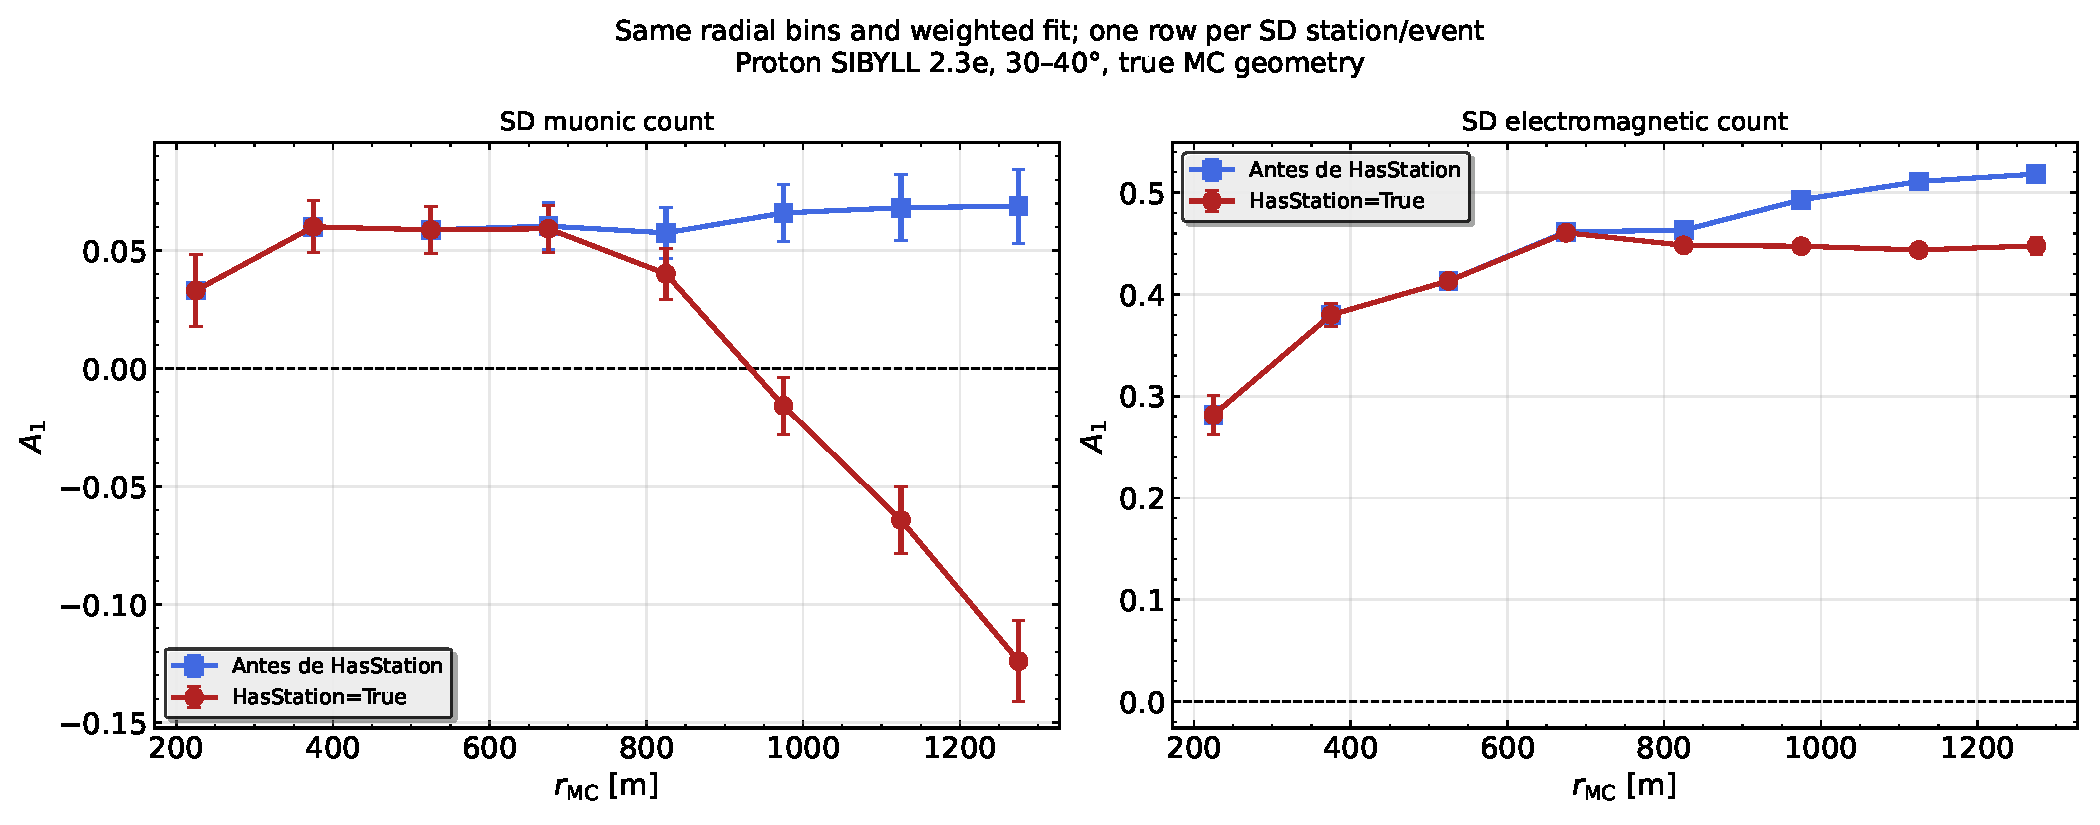
\includegraphics[width=\textwidth]{claude_work/revision_asimetrias_sd_umd/02_notebooks/02_reproduccion/resultados/SD_antes_despues_mismos_bins.pdf}
\caption{Control de la selección SD con geometría Monte Carlo y el mismo bineado radial y azimutal a ambos lados del corte. El conteo muónico permanece positivo antes de exigir \texttt{HasStation} e invierte su signo después. La componente electromagnética permanece positiva, aunque su amplitud también cambia. Las barras de esta figura reproducen los errores formales del ajuste ponderado original; la Tabla~\ref{tab:infill2026_comparacion} utiliza incertidumbres por remuestreo de lluvias.}
\label{fig:infill2026_antes_despues}
\end{figure}

El resultado del intervalo exterior se resume en la Tabla~\ref{tab:infill2026_comparacion}. Se conserva el conteo UMD de la selección original como referencia, sin presentarlo como una muestra subterránea no seleccionada.

Las incertidumbres de esta comparación se obtienen mediante $1200$ réplicas
pareadas sobre $960$ grupos de lluvia progenitora identificados en la muestra.
En cada réplica se mantienen juntas sus reutilizaciones y se recalculan las
medias azimutales, sus errores y el ajuste para los tres observables. Este
agrupamiento utiliza los identificadores disponibles y no sustituye una
auditoría completa de la genealogía de las simulaciones.

\begin{table}[H]
\centering
\begin{tabular}{lcc}
\toprule
Observable y selección & $A_1$ & $\sigma_{\mathrm{bootstrap}}$\\
\midrule
SD muónico antes de \texttt{HasStation} & $+0.0689$ & $0.0157$\\
SD muónico con \texttt{HasStation} & $-0.1240$ & $0.0186$\\
UMD, selección original & $+0.0816$ & $0.0344$\\
\bottomrule
\end{tabular}
\caption{Comparación para $1200\leq r<1350$~m y $30^\circ\leq\theta<40^\circ$. Las incertidumbres son desviaciones estándar de un \textit{bootstrap} que conserva conjuntamente las estaciones, módulos y reutilizaciones agrupadas por identificador de lluvia progenitora. No son las incertidumbres formales del ajuste a medias independientes. Los coeficientes no deben confundirse con valores ilustrativos citados anteriormente a radio nominal $r\simeq1200$~m y con otro bineado.}
\label{tab:infill2026_comparacion}
\end{table}

En esta corona el conjunto SD pasa de $12212$ a $3694$ registros al aplicar la condición. El cambio de signo se obtiene sin modificar sus conteos, sus coordenadas Monte Carlo ni el estimador. Por lo tanto, la selección es suficiente para producir la inversión observada en esta muestra. No es necesario introducir un nuevo término atmosférico negativo para explicar la diferencia entre esos dos promedios.

La comparación con UMD tampoco debe reducirse a que ambos coeficientes anteriores al corte sean positivos. En el intervalo de la tabla, la diferencia pareada SD antes del corte menos UMD es $-0.0127$, con intervalo percentil puntual del $95\%$ de $[-0.0897,+0.0555]$. No se resuelve allí una diferencia con ese procedimiento, pero ello no prueba igualdad física. En coronas interiores sí aparecen diferencias, por lo que retirar \texttt{HasStation} no vuelve idénticas las curvas de ambos instrumentos. El remuestreo contempla la dependencia entre registros de una lluvia, no las incertidumbres sistemáticas del detector o del modelo hadrónico.

\subsubsection{Interpretación física: selección dependiente de la señal}

Una hipótesis coherente con el signo observado es el acoplamiento entre la componente electromagnética y la condición que retiene una estación. En la región temprana, una contribución electromagnética mayor puede ayudar a retener estaciones aun con pocos muones. En la tardía, con menor contribución electromagnética, las estaciones que sobreviven pueden estar enriquecidas en fluctuaciones muónicas positivas. El promedio de muones por estación retenida puede resultar entonces mayor en la región tardía, aunque el promedio previo favorezca la temprana.

La atenuación electromagnética participaría así de forma indirecta, modificando la señal que favorece la selección; no cambia el signo de las pérdidas pasivas de muones. Tampoco se confunden electrones con muones: cambia el conjunto de estaciones en el que se promedian los muones verdaderos.

El cambio de signo al aplicar \texttt{HasStation} es un resultado del control. La secuencia particular de ayuda electromagnética y enriquecimiento muónico es una interpretación física pendiente de aislamiento causal. \texttt{HasStation} informa presencia en la colección reconstruida y no identifica, por sí solo, un único umbral de disparo ni una etapa específica de reconstrucción. El resultado no demuestra un error del programa \textit{Offline}: una selección correctamente implementada puede sesgar una media si se la interpreta como incondicional.

\subsection{Qué establece la comparación con el UMD}
\label{subsec:umd_poblacion_seleccion}

El UMD y el SD no muestrean la misma apertura ni la misma población de cruces. El suelo modifica las distribuciones de energía y dirección de los muones que alcanzan los centelladores. Por otra parte, los muones contabilizados por el SD contribuyen directamente a la señal del tanque que interviene en la selección. Un muón que atraviesa un módulo enterrado cercano no es, en general, el mismo que atraviesa el tanque. La correlación de cada conteo con la selección SD puede, por ello, ser diferente, aun cuando ambos estén correlacionados por pertenecer a la misma lluvia.

Estas diferencias permiten comprender por qué no es obligatorio que el UMD reproduzca la inversión del SD seleccionado. No prueban que el UMD esté libre de selección ni que su exceso temprano sea exclusivamente atmosférico. La concordancia aproximada de un modelo de transporte y apertura con una amplitud UMD tampoco reemplaza el control de la población efectivamente observada.

Con los resúmenes disponibles no se ha construido una comparación UMD equivalente a la de la Figura~\ref{fig:infill2026_antes_despues}. La auditoría de los objetos ADST identificó que la verdad de los centelladores puede no quedar serializada cuando no se crean los canales electrónicos asociados al disparo SD. Un contador ausente o una suma sobre una lista vacía no demuestran que no hayan atravesado muones el módulo. Los ceros conservados por compatibilidad con el lector original no deben convertirse en ceros físicos de una población UMD no seleccionada. Recuperar más filas sin \texttt{HasStation} tampoco resuelve por sí solo esa falta de información.

\subsection{Geometría reconstruida: un sistemático distinto}
\label{subsec:infill_rec}

Se reemplazan ahora el núcleo y la dirección verdaderos por sus valores reconstruidos. Aun manteniendo las mismas estaciones, cambian el radio y el azimut asignados a cada una y pueden producirse migraciones entre coronas. Este efecto es distinto del anterior: la selección modifica qué estaciones entran, mientras que la reconstrucción geométrica modifica dónde se ubican las que entran.

En las comparaciones originales, el cambio de conteo MC a REC con geometría fija conserva gran parte de la tendencia del UMD. Al cambiar también las coordenadas, la extracción se degrada en varias regiones, especialmente cuando la amplitud es pequeña o el gradiente radial es grande. Las grillas con geometría reconstruida documentan ese comportamiento; no se asume que la pérdida sea uniforme ni que exista una ventana óptima universal.

Un modelo de errores de fase independientes del conteo y del azimut verdadero, simétricos y sin migración radial daría $A_1^{\mathrm{REC}}=A_1^{\mathrm{MC}}\langle\cos\Delta\phi\rangle$. Este límite ilustra una atenuación por mezcla angular, pero los errores reales del núcleo también tienen estructura direccional. En el control con estaciones del Infill mostrado en la presentación RAFA y en la Figura~\ref{fig:bias_core_azimut}, $\Delta r=r_{\mathrm{MC}}-r_{\mathrm{REC}}$ es negativo en la región temprana y positivo en la tardía. A dirección fija, el patrón es compatible con un desplazamiento del núcleo reconstruido hacia el lado tardío; las diferencias de dirección y las migraciones de muestra deben controlarse para cuantificarlo.

Una LDF que no representa explícitamente la modulación azimutal puede absorber parte de ella mediante ajustes de posición y de otros parámetros. Esta interpretación debe distinguirse del modelo de remuestreo de residuos de conteo de la Sección~\ref{subsec:toy_model}: ese modelo cuantifica cómo una respuesta direccional del conteo modifica $A_1$, pero no vuelve a ejecutar la reconstrucción del núcleo y no demuestra por sí solo toda la cadena causal propuesta para su desplazamiento.

La componente electromagnética puede seguir mostrando una modulación positiva significativa bajo geometría reconstruida. Una amplitud mayor y errores estadísticos menores facilitan su detección, pero la abundancia de partículas no elimina un sesgo de coordenadas. Asimismo, la persistencia de un coeficiente SD negativo no exige una población de muones blandos con proyección negativa: la muestra sigue condicionada por selección, y la geometría reconstruida puede modificar ese coeficiente sin eliminar su signo.

\subsection{Alcance de los resultados y controles restantes}
\label{subsec:comparacion_performance_umd}
\label{subsec:fast_mc}

Una evaluación MC--REC completa debe comparar, sobre una muestra emparejada, el cambio de conteo a geometría fija y el cambio de geometría a conteo fijo. Las diferencias de amplitud deben incluir sus covarianzas y las migraciones radiales; un cociente resulta inestable cuando el coeficiente de referencia es cercano a cero. En presencia de sesgos correlacionados, ni $A_1^{\mathrm{REC}}$ es una cota inferior universal ni $A_1^{\mathrm{MC}}$ una cota superior universal.

El resultado central de este capítulo es que la condición de presencia de estación reconstruida induce la inversión del promedio muónico SD en la muestra auditada. La física de propagación, la proyección y la respuesta del tanque siguen siendo necesarias para predecir las poblaciones y sus señales; la selección debe aplicarse además para predecir el observable realmente ajustado. No se establece una inversión universal del flujo al suelo ni un fallo de reconstrucción instrumental.

Los controles siguientes tienen requisitos de información diferentes. Extender la prueba SD a otros primarios, energías e inclinaciones requiere repetir la comparación sobre sus estaciones simuladas. Separar las etapas responsables de la selección requiere sus estados de disparo, lectura y reconstrucción junto con conteos y señales. Para obtener el control UMD se necesita conservar el conteo anterior a la electrónica, distinguiendo explícitamente cero de dato ausente. Ninguna de estas preguntas exige cinemática individual de producción.

En cambio, una predicción desde producción necesita la distribución conjunta de profundidad, energía y momento transversal, con sus correlaciones y su transporte hasta los detectores \cite{Cazon2012}. Esa información no puede reconstruirse únicamente a partir de los conteos agregados de los ADST. El propagador fenomenológico previo no resolvió esa limitación y no constituye una validación de la antigua explicación de muones blandos. La sensibilidad a composición y energía del Infill, así como la transferencia a datos reales, quedan sujetas a controles propios; no se deducen automáticamente del resultado favorable del Anillo Denso ni de la prueba de selección presentada aquí.

\newpage

\clearpage
\section*{Anexos citados de la tesis original}
Esta vista previa contiene sólo los tres capítulos propuestos. Las
referencias siguientes identifican anexos del manuscrito original, que
no se modifican ni se reproducen aquí.
\phantomsection
\makeatletter\def\@currentlabel{A}\makeatother
\label{anexo:ajustes_anillo_denso}
\paragraph*{Anexo A: Ajustes armónicos para el Anillo Denso.}
La grilla de ajustes permanece en el capítulo de anexos de la tesis.
Su discusión de valores elevados de $\chi^2$ deberá armonizarse con el
criterio estadístico del nuevo capítulo 5 antes de integrar los borradores.
\phantomsection
\makeatletter\def\@currentlabel{B.1}\makeatother
\label{anexo:ajustes_infill_mc}
\paragraph*{Anexo B.1: Grillas del Infill con geometría Monte Carlo.}
Las grillas originales se mantienen como material de referencia. No son
un nuevo control de estaciones anterior a la selección SD.
\clearpage
\printbibliography[heading=bibintoc,title={Referencias}]
\end{document}
